\vspace{-.5em}
\section{Results}
\label{exp}
We evaluate SVC first on a single node MySQL database to evaluate its accuracy, performance, and efficiency in a variety of materialized view 
scenarios.
We look at three main applications, join view maintenance, aggregate view maintenance, and a data cube application, on the standard TPCD benchmark 
and skewed version of the benchmark TPCD-Skew.
Then, we evaluate the outlier indexing approach in terms of improved query accuracy and also evaluate the overhead associated with using the index.
After evaluation on the benchmark, we present an end-to-end application of log analysis with a dataset from a video streaming company.
In this application, we look at the real query workload of the company and materialize views that could improve performance of these queries.
We implement SVC in Spark 1.1 and deploy it on a 10-node cluster to analyze 1TB of logs.

\subsection{Single-node Experimental Setup}
Our single node experiments are run on a r3.large Amazon EC2 node (2x Intel Xeon E5-2670, 15.25 GB Memory, and 32GB SSD Disk) with a MySQL version 5.6.15 database.
These experiments evaluate views from 10GB TPCD and TPCD-Skew datasets.
TPCD-Skew dataset \cite{tpcdskew} is based on the Transaction Processing Council's benchmark
schema but is modified so that it generates a dataset with values drawn from a Zipfian distribution instead of uniformly.
The Zipfian distribution \cite{mitzenmacher2004brief} is a long-tailed distribution with a single parameter $z=\{1,2,3,4\}$ which a larger
value means a more extreme tail.
$z=1$ corresponds to the basic TPCD benchmark. 
We implement incremental view maintenance with a \textbf{update...on duplicate key insert} command.
We implement SVC's sampling operator with a linear hash writter in C that is evoked in MySQL as a stored procedure.
In all of the applications, the updates are kept in memory in a temporary table, and we discount this loading time from our experiments.

Below we describe the view definitions and the queries on the views:

\textbf{Join View: } In the TPCD specification, two tables recieve insertions and updates: \textbf{lineitem} and \textbf{orders}.
Out of 22 parameterized queries in the specification, 12 are group-by aggregates of the join of \textbf{lineitem} and \textbf{orders} (Q3, Q4, Q5, Q7, Q8, Q9, Q10, Q12, Q14, Q18, Q19, Q21).
Therefore, we define a materialized view of the foreign-key join of \textbf{lineitem} and \textbf{orders}, and compare incremental view maintenance and SVC.
We treat the 12 group-by aggregates as queries on the view.

\textbf{Data Cube: } Another application which is common in industry analytics is data cubing.
We define the following ``base cube" as a materialized view that calculates the total revenue 
grouped by distinct customer, nation, region, and part number.
\begin{lstlisting}
select
  sum(l_extendedprice * (1 - l_discount)) as revenue,
  c_custkey, n_nationkey,
  r_regionkey, L_PARTKEY
from
  lineitem, orders,
  customer, nation,
  region
where
  l_orderkey = o_orderkey and
  O_CUSTKEY = c_custkey and
  c_nationkey = n_nationkey and
  N_REGIONKEY = r_regionkey

group by
  c_custkey, n_nationkey, 
  r_regionkey, L_PARTKEY
\end{lstlisting}
The queries on this view are ``rollup" queries that aggregate over 
subsets of the groups (eg. total of all customers in North America).
\reminder{todo}

\textbf{Queries as Views: } Finally, to test the generality of SVC, we treat each of the 22 queries in TPCD as a materialized view.
10 out of the 22 can benefit from SVC (see table ??).
\reminder{todo}
As each of the queries are actually parameterized queries, we generated 10 views for each TPCD query.
For each of the views, we generated \emph{queries on the views}.
We generated 100 random aggregate queries for each view.
We detail the incremental maintenance procedures in ??.

\subsubsection{Distributed Experimental Setup}
We evaluated performance on Apache Spark 1.1.0 with a 10 node r3.large Amazon EC2 cluster.
Spark supports materialized views through a distributed data structure called an RDD \cite{zaharia2012resilient}.
There is a SQL interface which transforms the RDD's using Map-Reduce chains.
As RDD's are an immutable data structure, any maintenance must be done synchronously.
As Spark aslo does not have support for indices, we rely on partitioned joins for incremental maintenance of the views.
We partitioned the views by primary-by key, and apply a full outer join of the updates with the partitioned view.

We evalaute SVC on a 1TB dataset of logs from Conviva \cite{conviva}.
Conviva is a video streaming company and we evaluated our approach on user activity logs.
1TB corresponded to a sample of customer data from 1 year of logs.
With this dataset, there was a corresponding dataset of analyst SQL queries on the log table.
We used this dataset to evaluate the end-to-end accuracy and performance of the system in a real-world application.

Using the dataset of analyst queries, we identified 8 common summary statistics-type queries that calculated engagement and error-diagnosis metrics for specific customers on a certain day.
We generalized these queries by turning them into group-by queries over customers and dates; that is a view that calculates the metric for every customer on every day.
We generated aggregate random queries over this dataset by taking either random time ranges or random subsets of customers.

\subsubsection{Metrics and Evaluation}
We evaluate SVC against the following alternatives:
\begin{itemize}
\item No maintenance: The baseline for evaluation is not applying any maintenance to the materialized view.
\item Incremental View Maintenance (IVM): Applying maintaining the full materialized view
\item SAQP: Maintaining a sample of the materialized view (using SVC) but estimating the result with AQP rather than using 
a correction.
\end{itemize}
Since both SAQP and SVC have sampling parameters, we denote a sample size of $x \% $ as SVC-x/SAQP-x.

To evaluate accuracy and performance, we define the following metrics:
\begin{itemize}
\item Relative Error: For a query result $r$ and an incorrect result $r'$, the relative error is \[\frac{\mid r-r' \mid}{r}\]. 
When a query has multiple results (a group-by query), then, unless otherwise noted, relative error is defined as the median over all the errors.
\item Maintenance Time: We define the maintenance time as the time needed to produce the up-to-date view for incremental view maintenance, and the time needed to produce the up-to-date sample in SVC. 
\end{itemize}

To illustrate how SVC gives the user access to this new tradeoff space, we will illustrate that SVC is more accurate than SAQP and No maintenance as a baseline; but is less computationally intensive than full IVM. 

\subsection{Single-node Accuracy and Performance}

\subsubsection{Join View}

\begin{figure}[t]
\centering
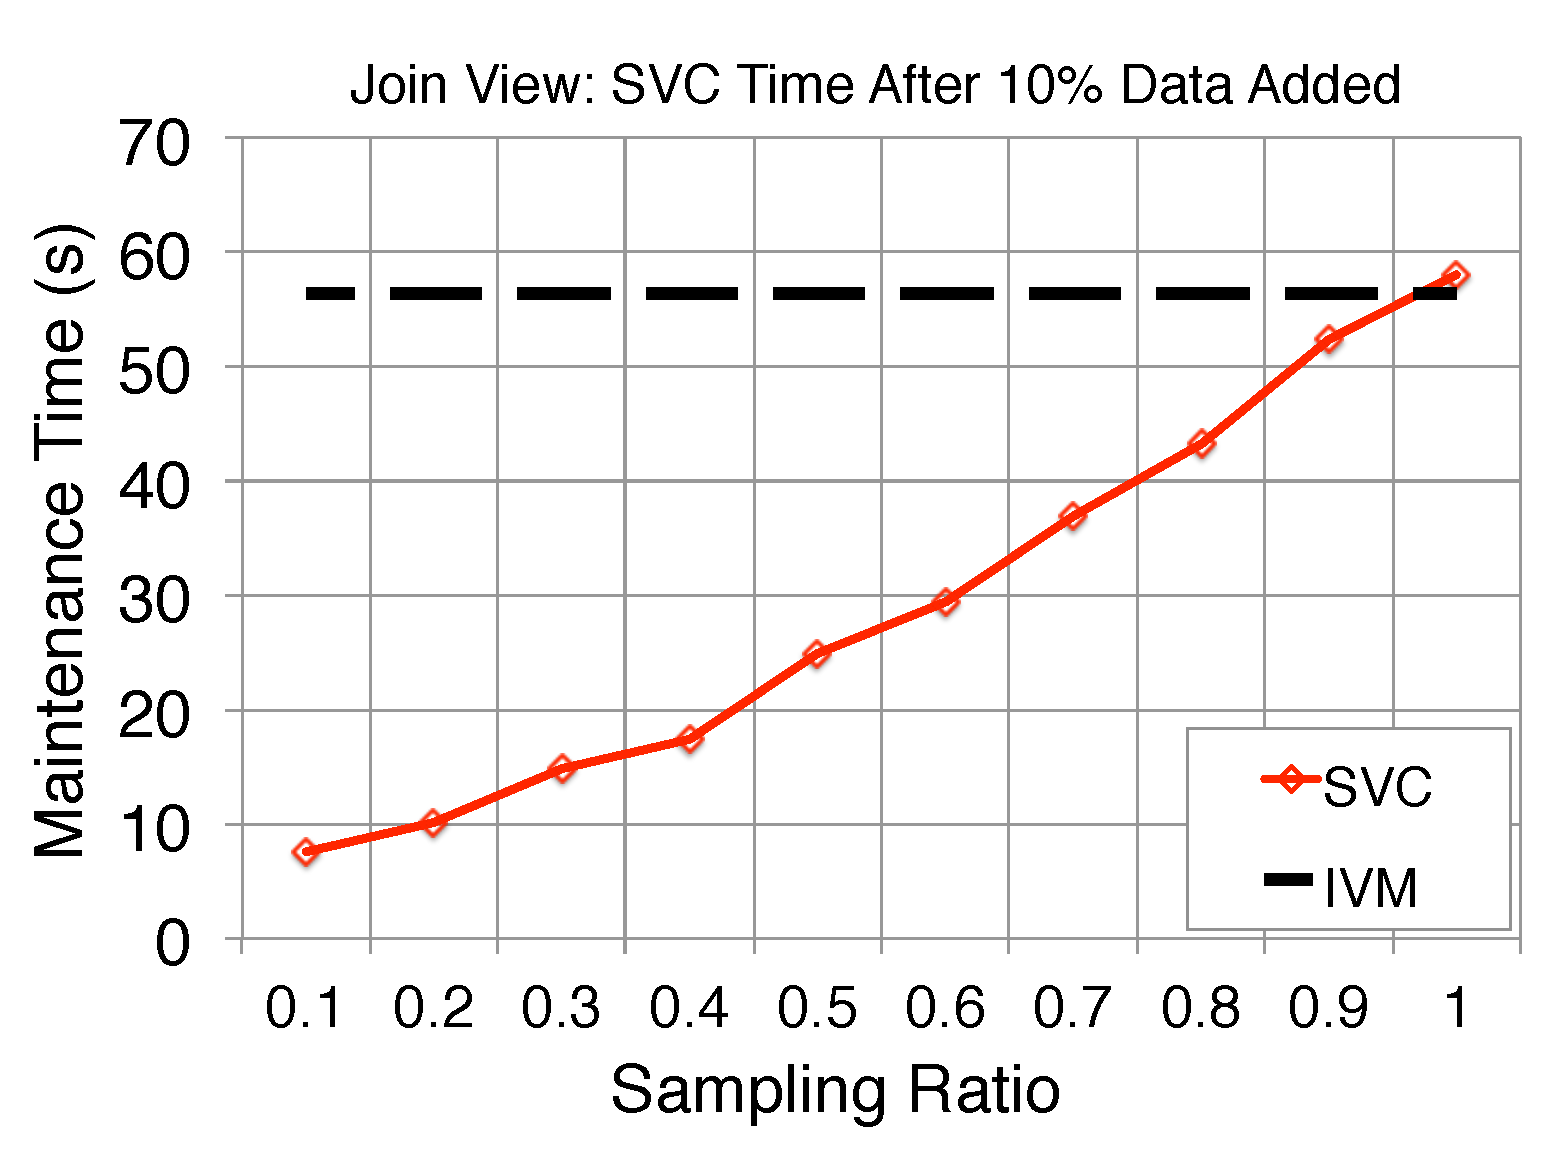
\includegraphics[scale=0.15]{exp/msj_1.pdf}
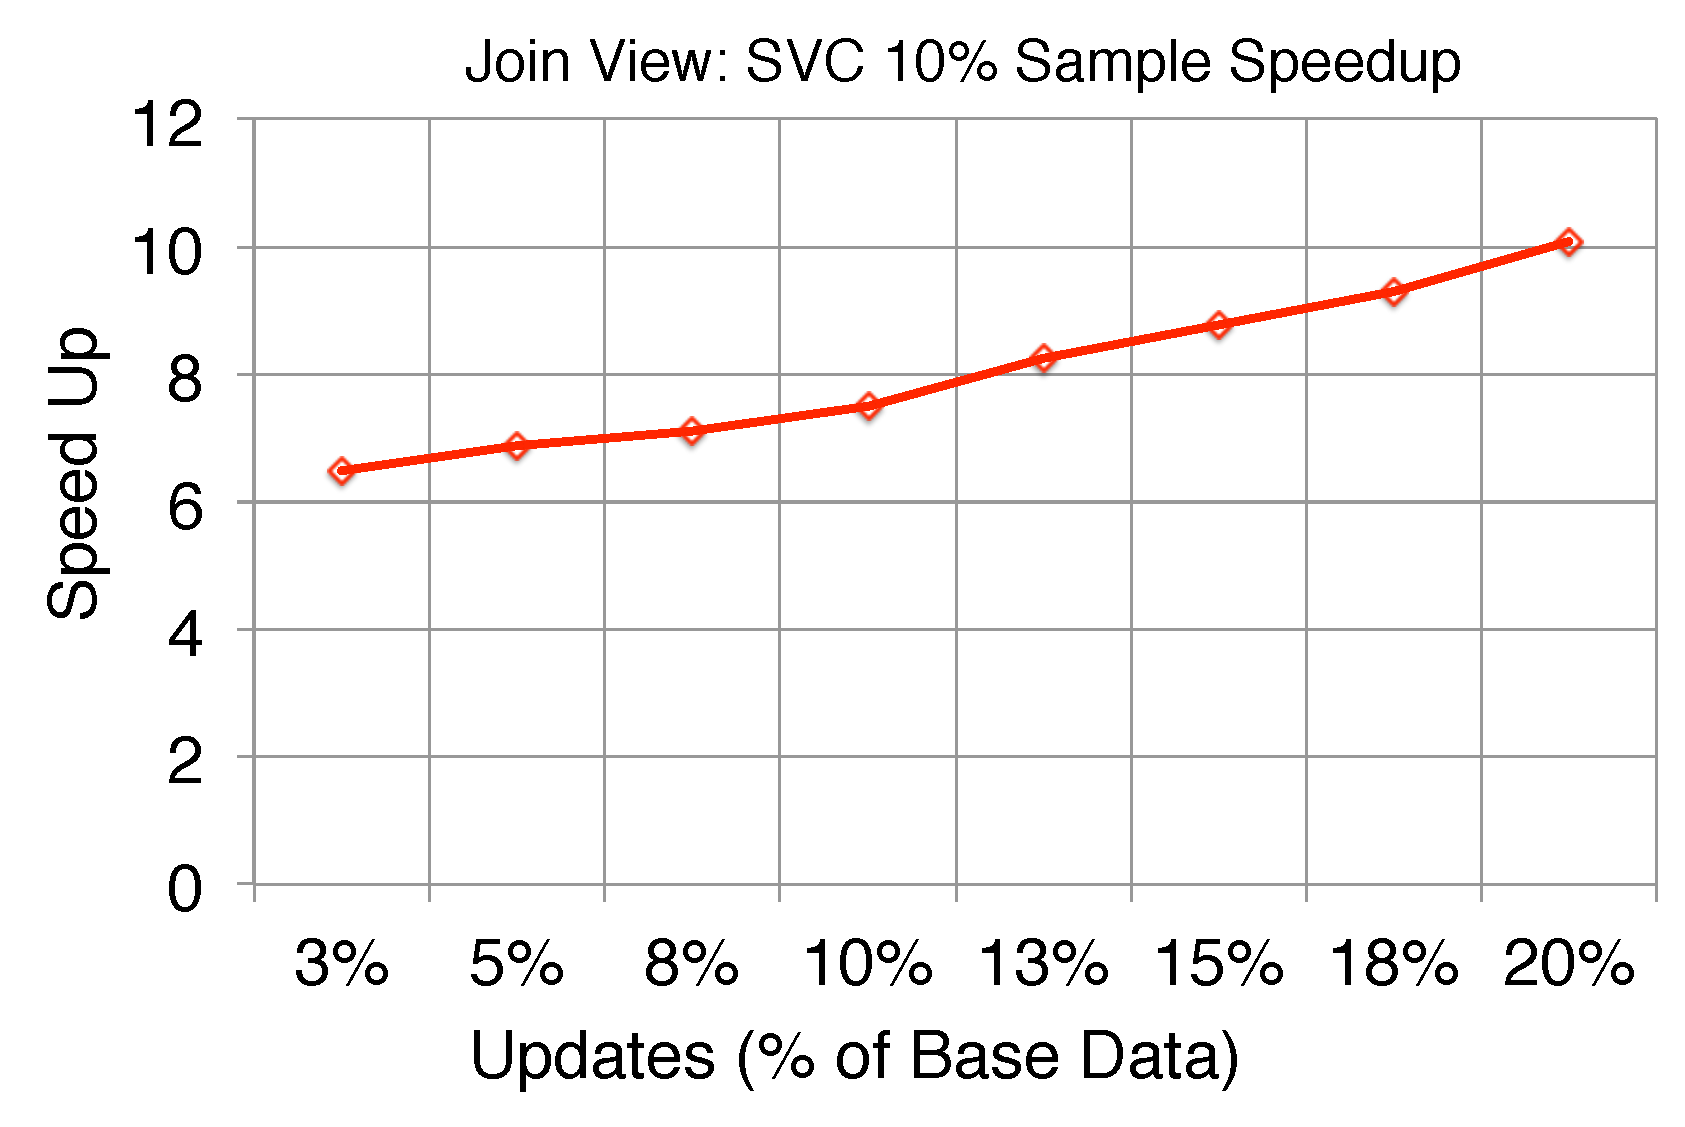
\includegraphics[scale=0.15]{exp/msj_2.pdf}
 \caption{TODO \label{exp-1-samplesize}}
\end{figure}

\begin{figure}[t]
\centering
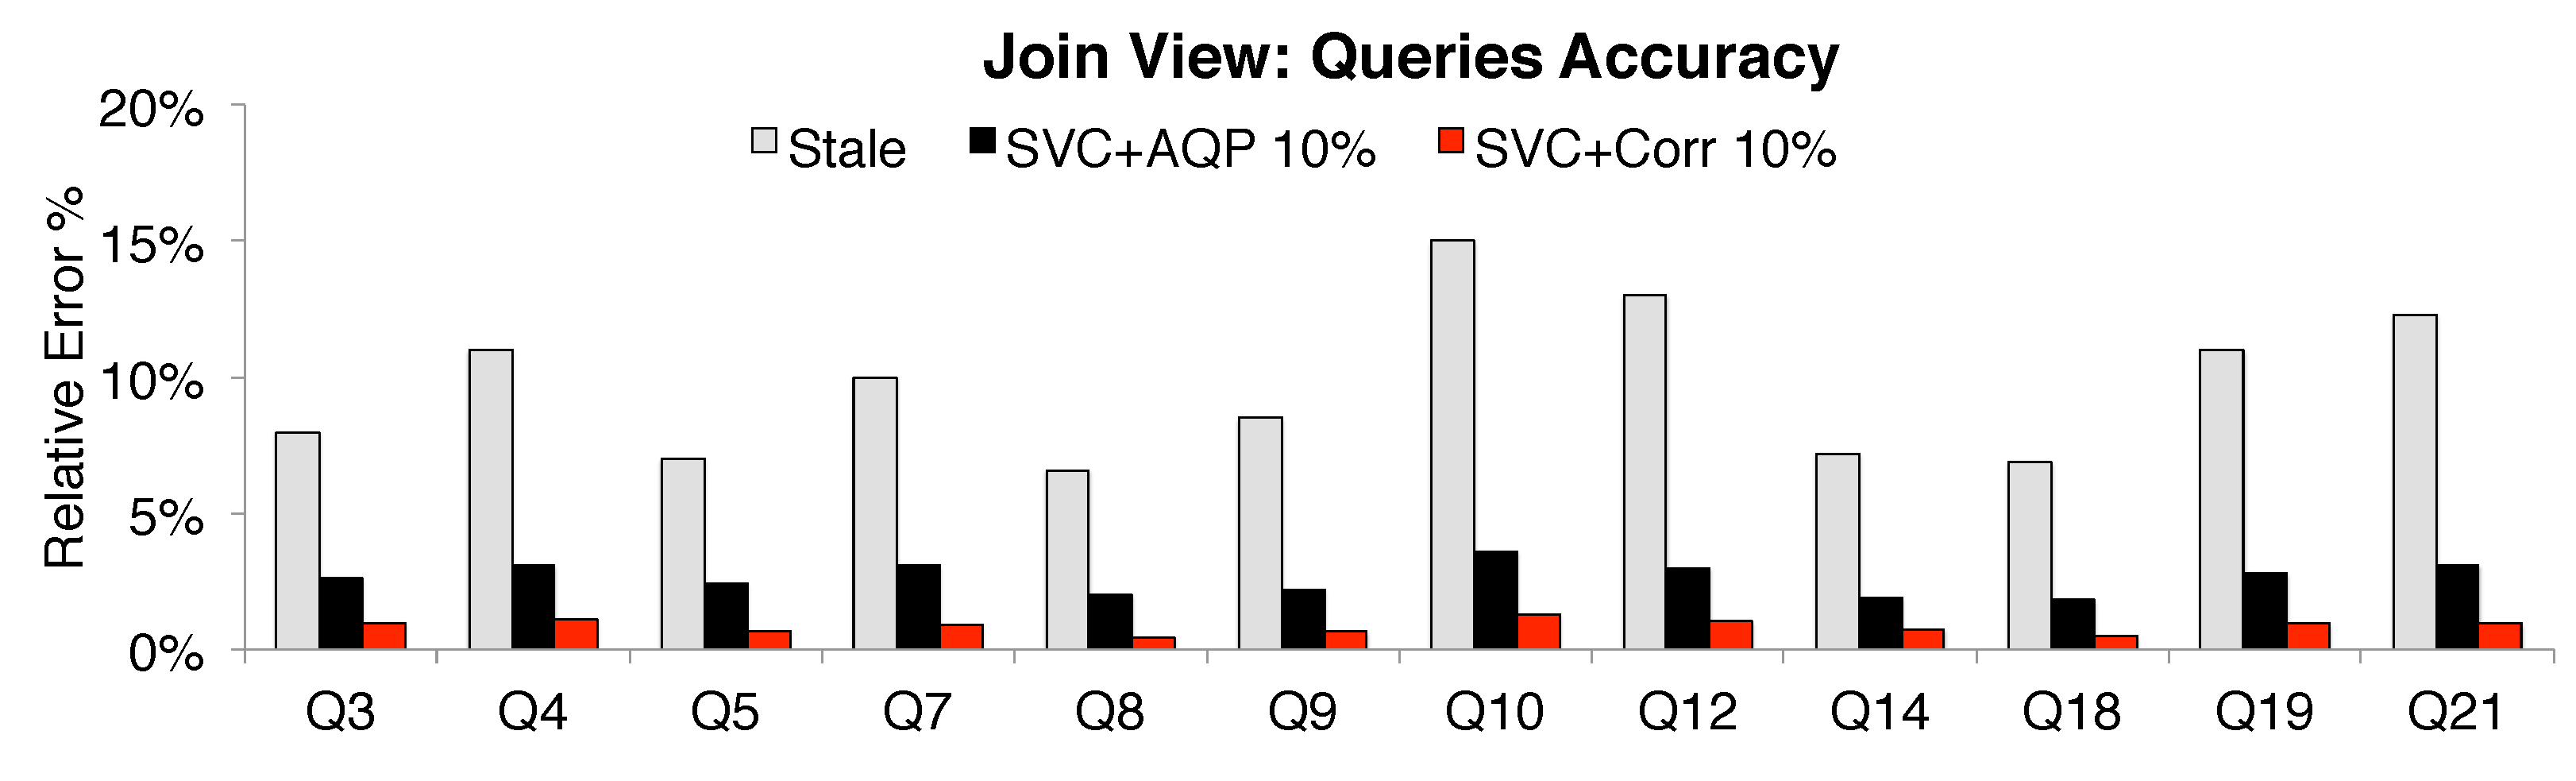
\includegraphics[scale=0.16]{exp/msj_3.pdf}
 \caption{TODO \label{exp-1-acc}}
\end{figure}

\begin{figure}[t]
\centering
 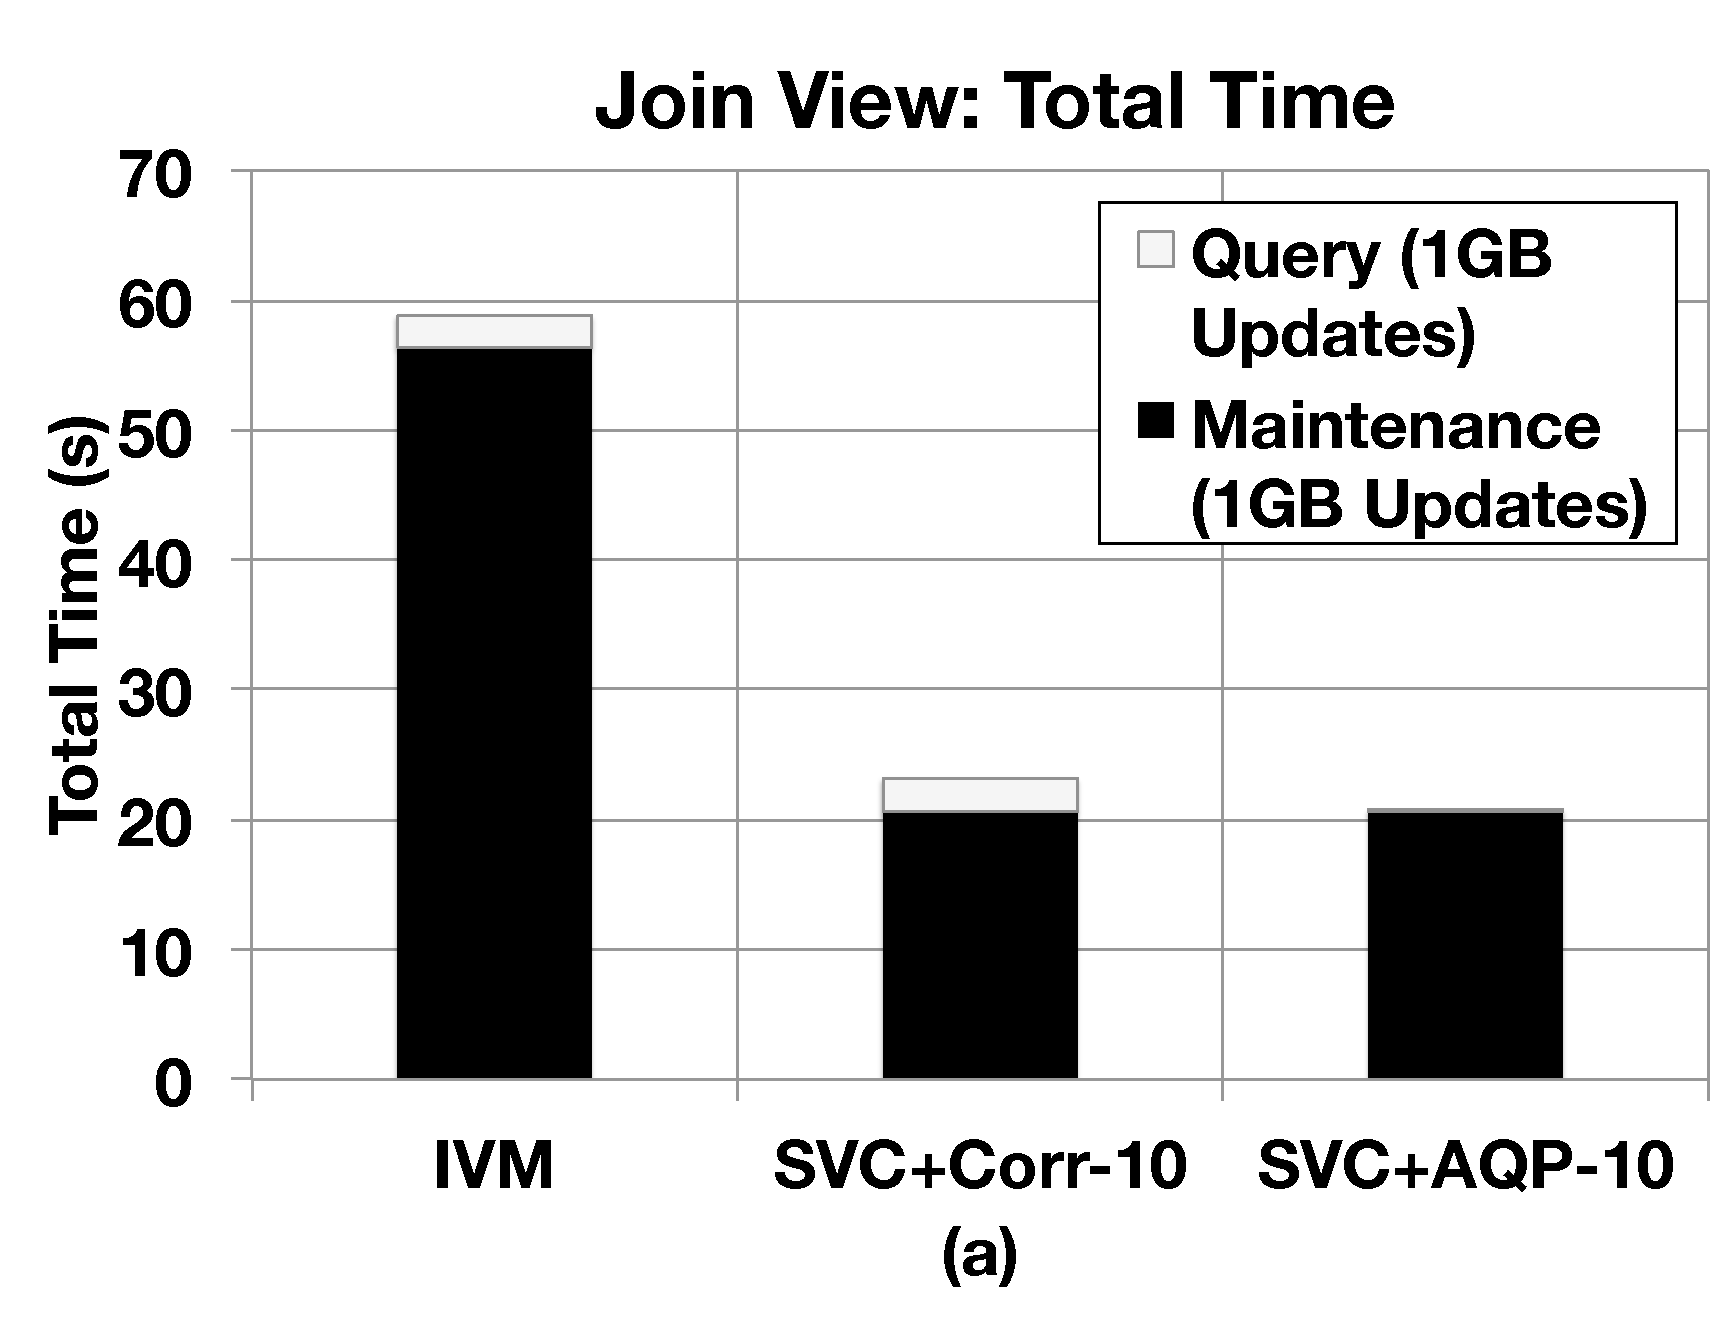
\includegraphics[scale=0.16]{exp/msj_4.pdf}
  \caption{TODO \label{exp-1-total}}
\end{figure}

\begin{figure}[t]
\centering
  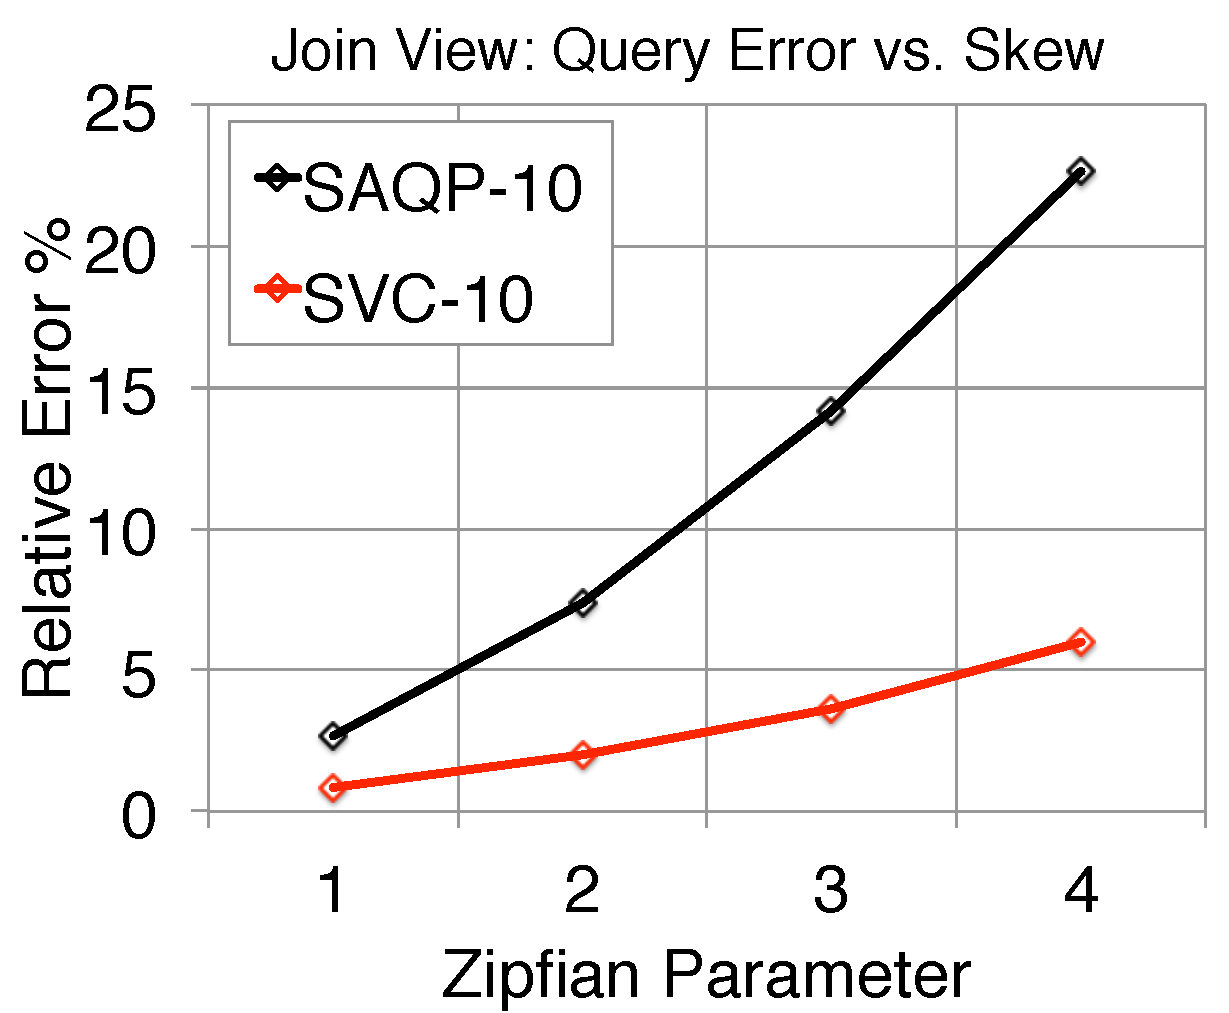
\includegraphics[scale=0.15]{exp/msj_5.pdf}
 \caption{TODO \label{exp-1-zipf}}
\end{figure}

In our first experiment, we evaluate how SVC performs on a materialized view of the join of \textbf{lineitem} and \textbf{orders}.
We generate a 10GB base TPCD dataset with skew $z=1$, and derive the view from this dataset.
We first generate 1GB (10\% of the base data) of updates (insertions and updates to existing records), and vary the sample size.
Figure \ref{exp-1-samplesize} a, shows the maintenance time of SVC as a function of sample size.
In black, we note the time for full IVM.
For this materialized view, sampling allows for significant savings in maintenance time; albeit for approximate answers.
In Figure \ref{exp-1-samplesize} b, we fix the sample size to 10\% and plot the speed up of the sample compared to IVM while varying the size of the updates.
For small update sizes, the speedup is far from ideal (5.3x at 250MB) but as the updates get larger the efficiency improves and in fact we observe super linearity (> 10x) at larger sizes.
This is likely due to the fact that while the base relations have a join-index, we do not create an index on the updates, making the join very expensive if there are large number of new records.

At the same design point with a 10\% sample, we evaluate the accuracy of SVC.
In Figure \ref{exp-1-acc}, we apply the TPCD queries.
A subset of these queries benefit from the materialized join and can be supported by our framework.
We found that SVC was 11.7x more accurate than the stale baseline, and 3.1x more accurate than applying SAQP to the sample.

It is true that SVC's correction technique moves some of the computation from maintenance to query execution.
We evaluate this overhead in Figure \ref{exp-1-total}, where we compare the total time maintenance and query execution.
We find that while SVC requires more query time than SAQP since it corrects a stale query rather than justing using a sample, 
this time is small in comparison to the total savings. 

Finally in Figure \ref{exp-1-zipf}, we vary the Zipfian parameter and show how the accuracy of SVC and SAQP changes.
While both techniques are sensitive to skew, we find that the gap between SVC and SAQP widens for more skewed datasets.
We can make SVC even more accurate using the outlier indexing which we will evalute in the later sections.

\subsubsection{Data Cube View}

\begin{figure}[t]
\centering
 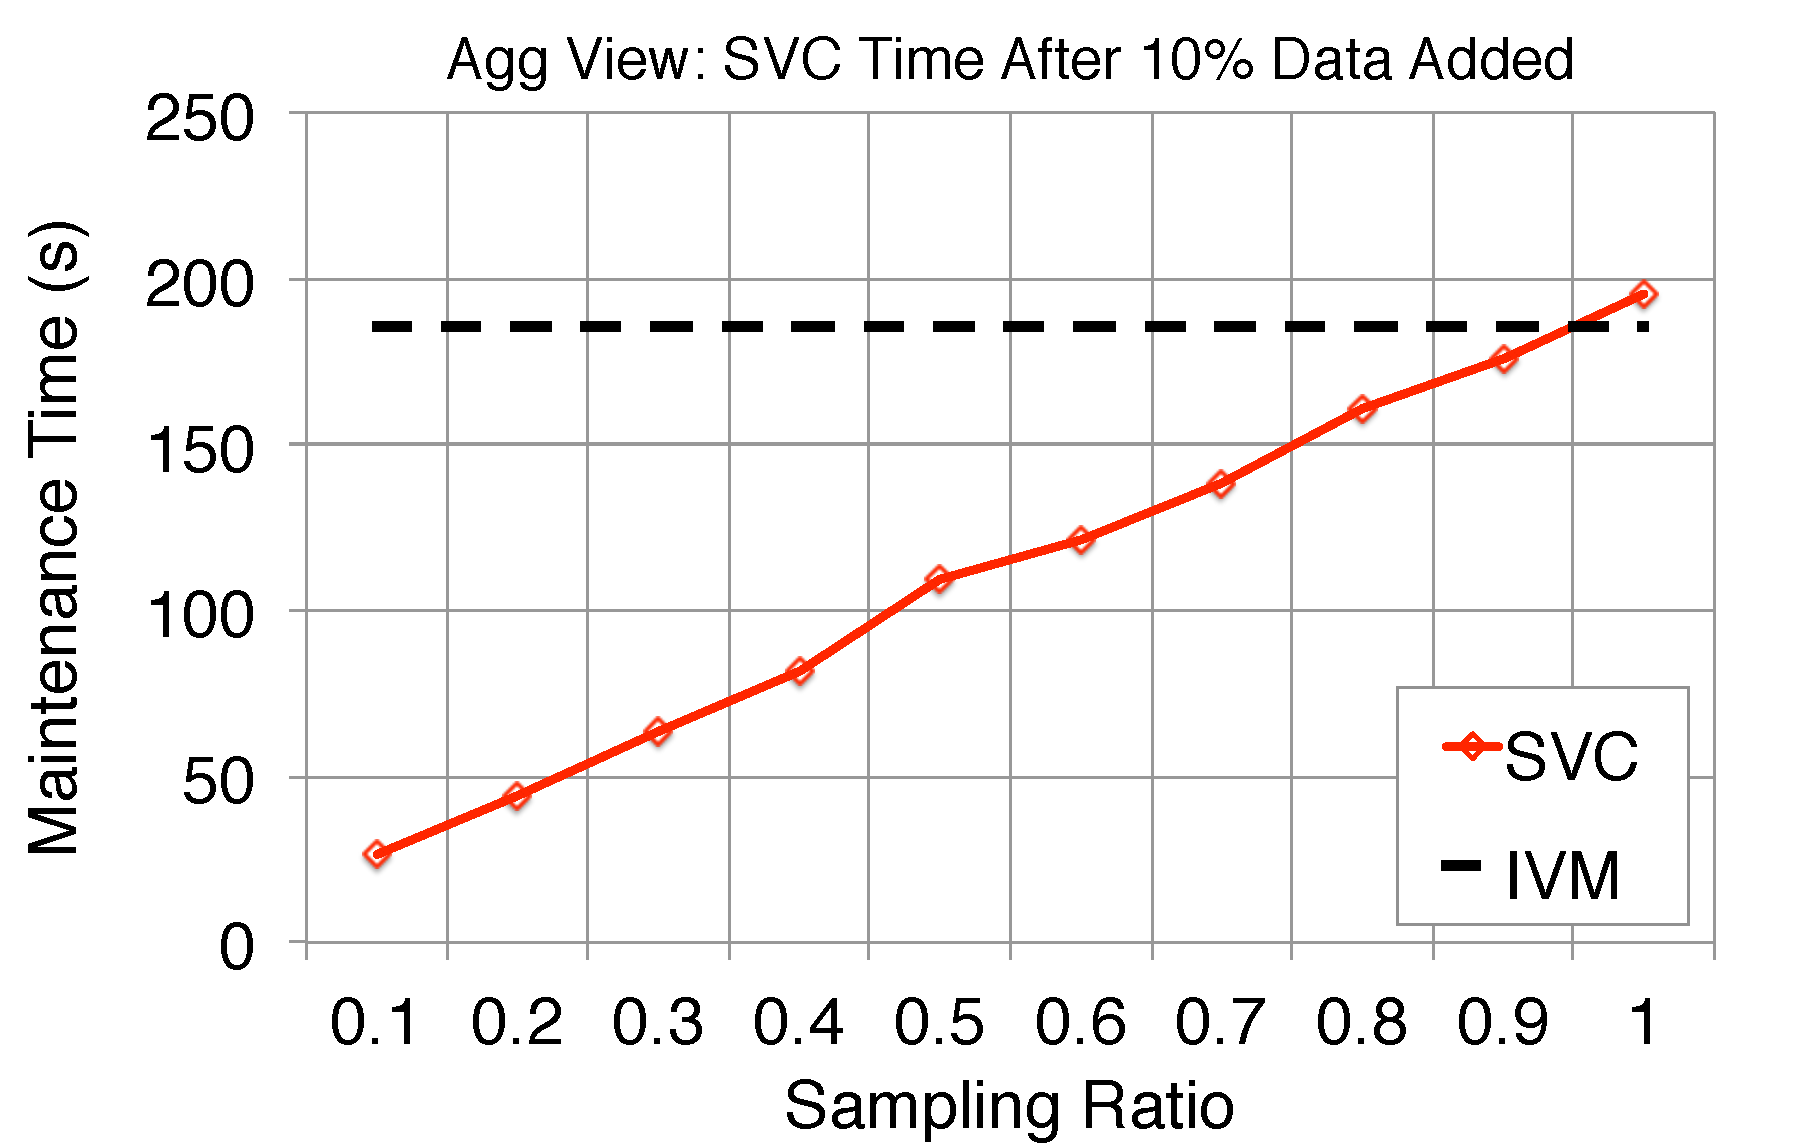
\includegraphics[scale=0.14]{exp/msdc_1.pdf}
 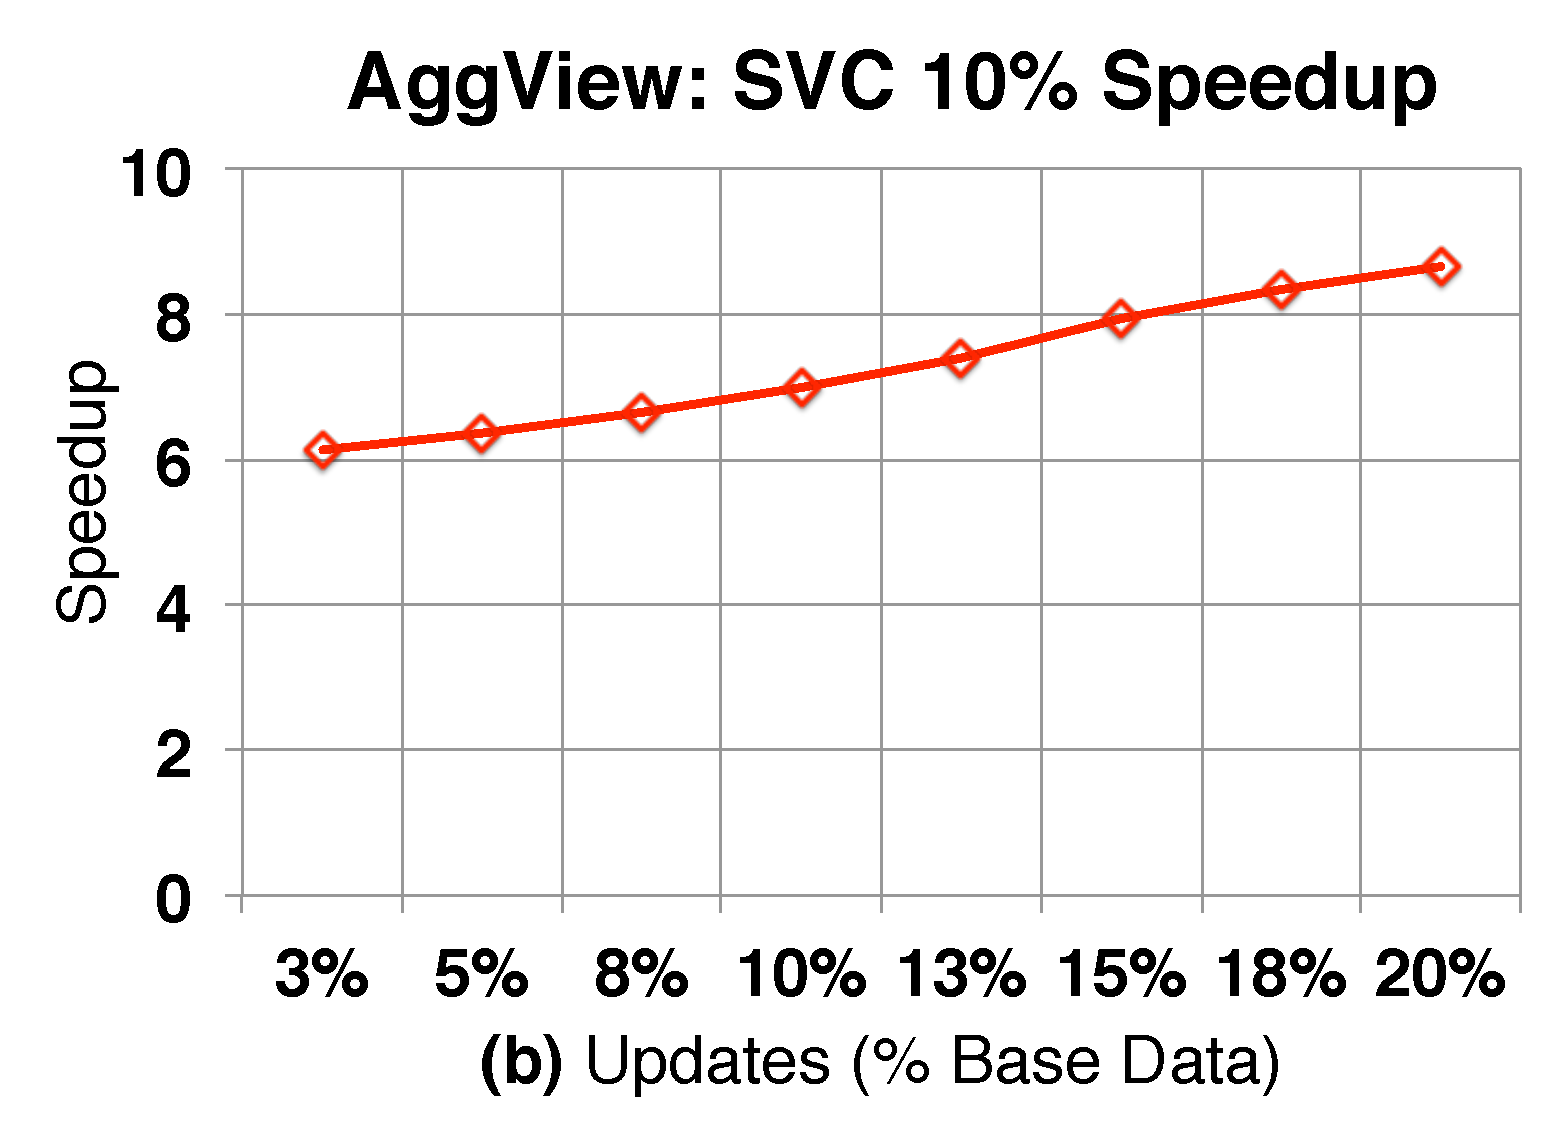
\includegraphics[scale=0.14]{exp/msdc_2.pdf}
  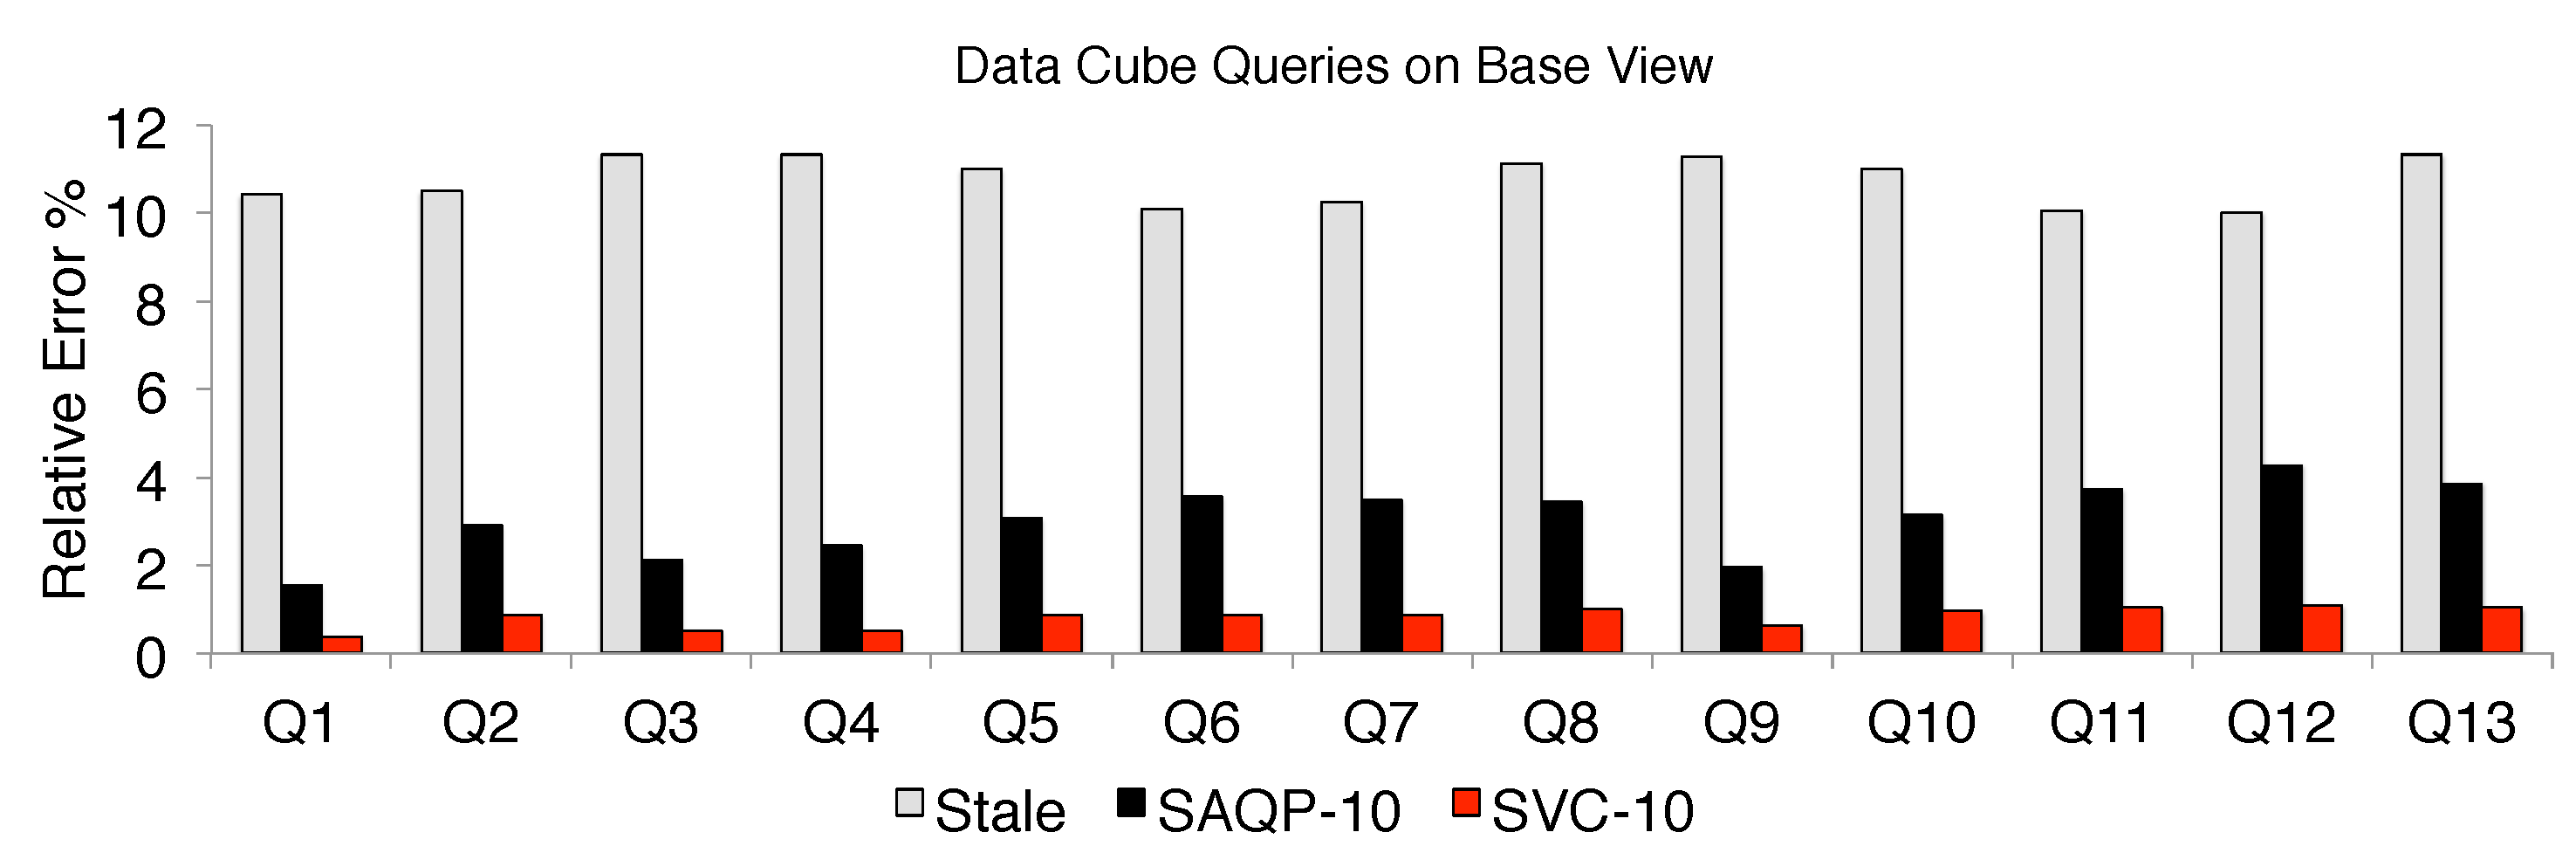
\includegraphics[scale=0.16]{exp/msdc_3.pdf}
   \caption{TODO \label{exp2-acc-sample}}
\end{figure}

\begin{figure}[t]
\centering
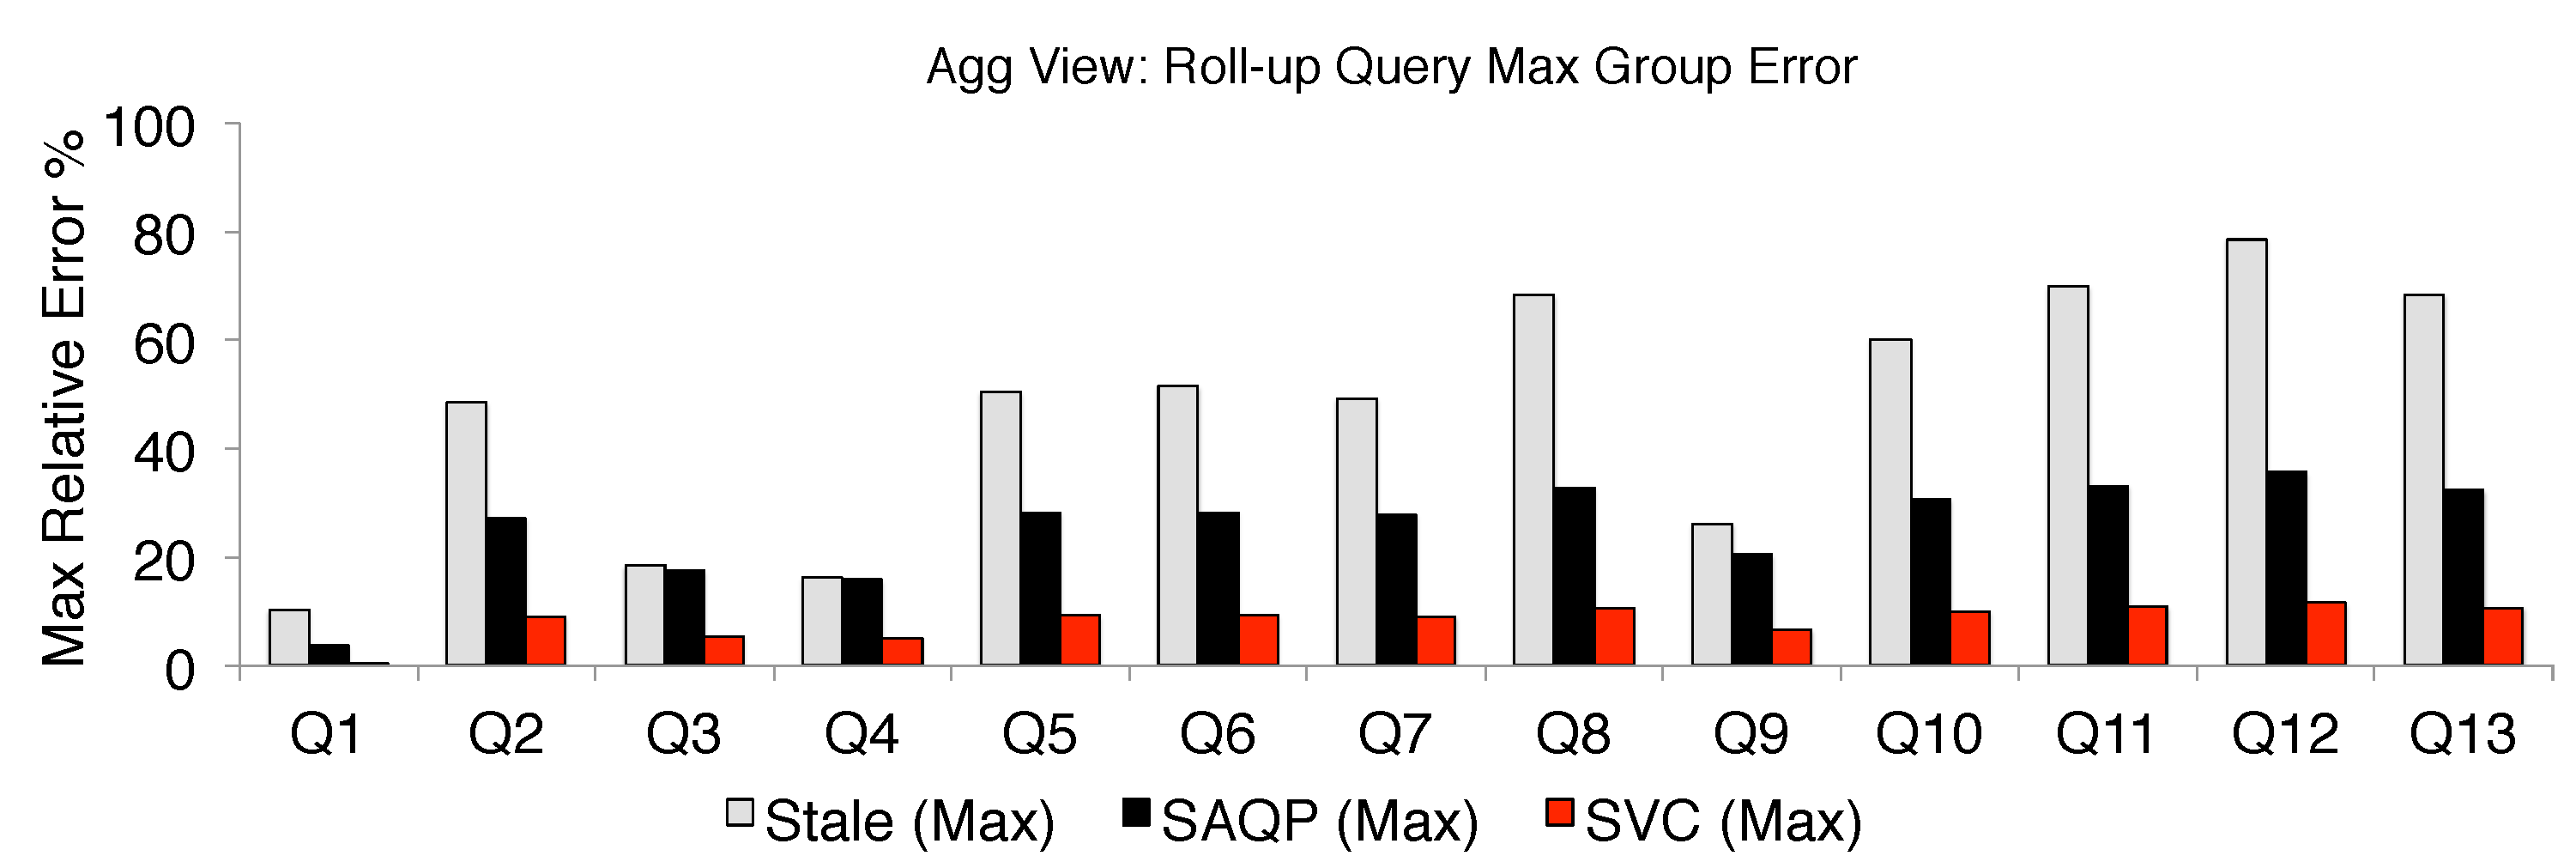
\includegraphics[scale=0.16]{exp/msdc_4.pdf}
   \caption{TODO \label{exp2-max}}
\end{figure}

\begin{figure}[t]
\centering
  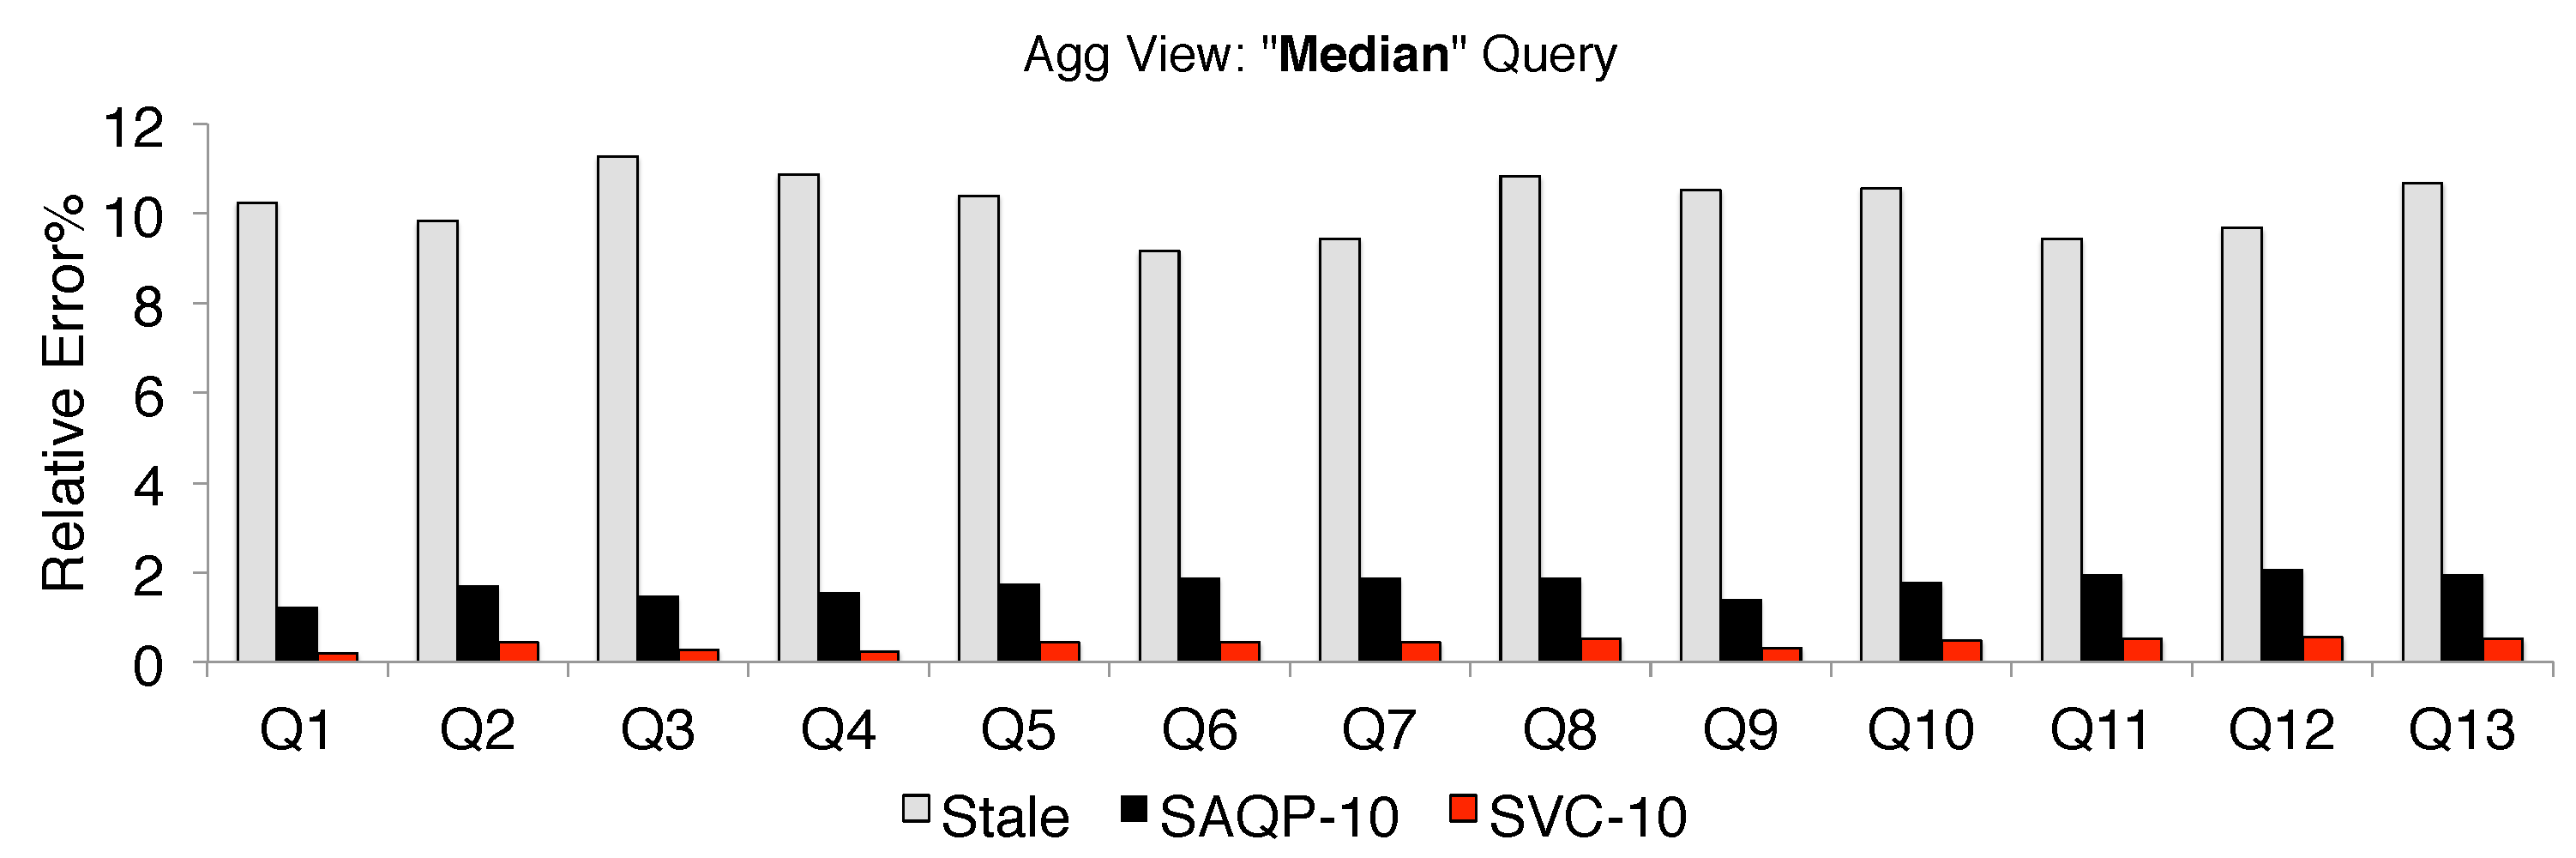
\includegraphics[scale=0.16]{exp/msdc_5.pdf}
  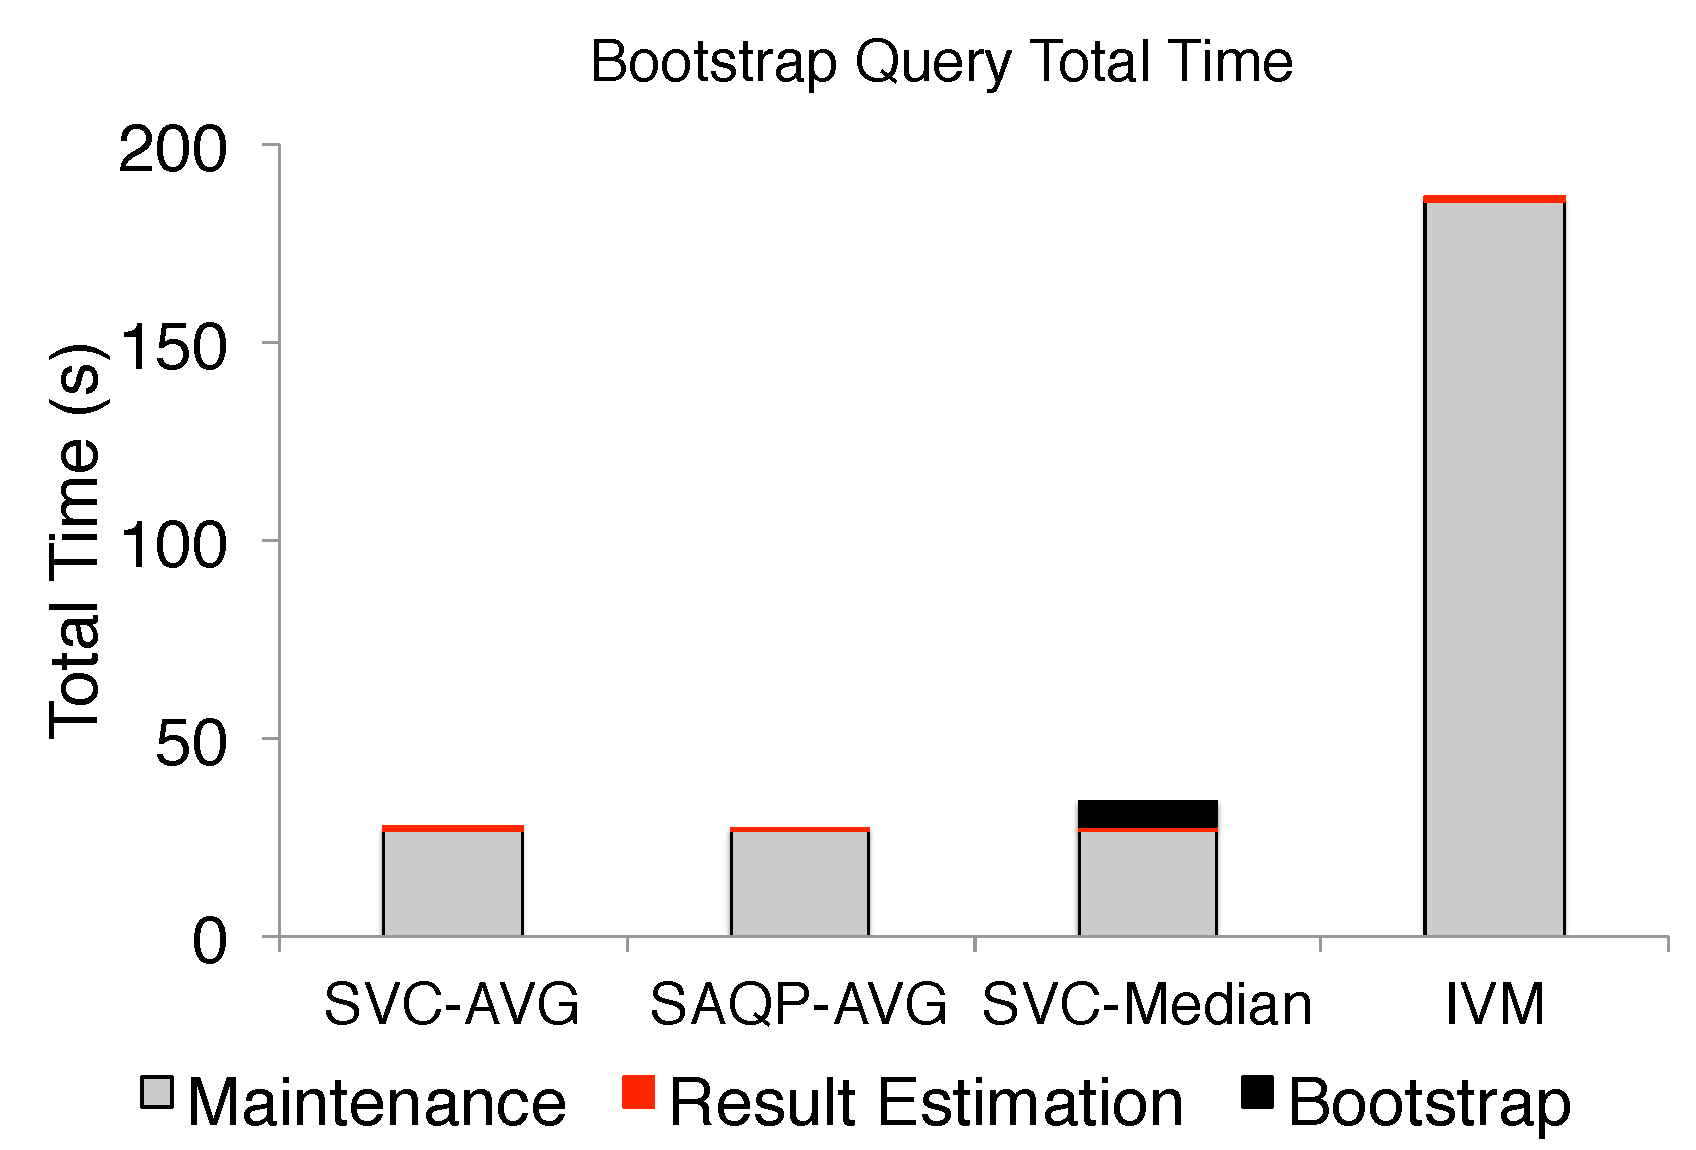
\includegraphics[scale=0.16]{exp/msdc_6.pdf}
 \caption{TODO \label{exp2-median}}
\end{figure}

Pre-computed joins are one important use case of materialization. 
Another application are data cubes.
Especially since our focus is on aggregate query processing, in the second experiment, we evaluate 
this use case in SVC.
We repeat our join experiment on the data cube defined before.
We generate a 10GB base TPCD dataset with skew $z=1$, and derive the base cube as a materialized view from this dataset.
We add 1GB of updates and apply SVC to estimate the results of all of the ``roll-up" dimensions.
We observed the same tradeoff where sampling significantly reduces the maintenance time; and when we fix the sample size at 10\%
and vary the update size we similarly observe that SVC tends towards an ideal efficiency (Figure \ref{exp2-acc-sample}).
At the sample size of 10\%, SVC is 12.9x more accurate than the stale baseline and 3.6x more accurate than SAQP.

Since the data cubing operation is primarily constructed by group-by aggregates, we can also measure the max error for each of the aggregates.
We see that while the median staleness is close to 10\%, for some queries some of the group aggregates have nearly 80\% error (Figure \ref{exp2-max}).
SVC greatly mitigates this error to less than 12\% for all queries.

Finally, we also use the data cube to illustrate how SVC can support a broader range of queries outside of \sumfunc, \countfunc, and \avgfunc.
We change all of the roll-up queries to use the \textbf{median} function (Figure \ref{exp2-median}).
First, both SVC and SAQP are more accurate as estimating the median than they were for estimating sums. 
This is because the median is less sensitive to variance in the data.
However, there is a nuance.
If we wish to calculate a confidence interval SAQP can apply an analytic form to calculate the confidence interval for the median, which SVC requires bootstrap to bound the error in the correction.
The statistical bootstrap is more computationally intensive than the analytic form, but the overhead is small compared to the total maintenance and query time.
There are techniques to speed up the calcuation of bootstrap using parallelization and single-pass sampling, and we defer this to future work.

\subsubsection{TPCD Query Views}

\begin{figure}[t]
\centering
 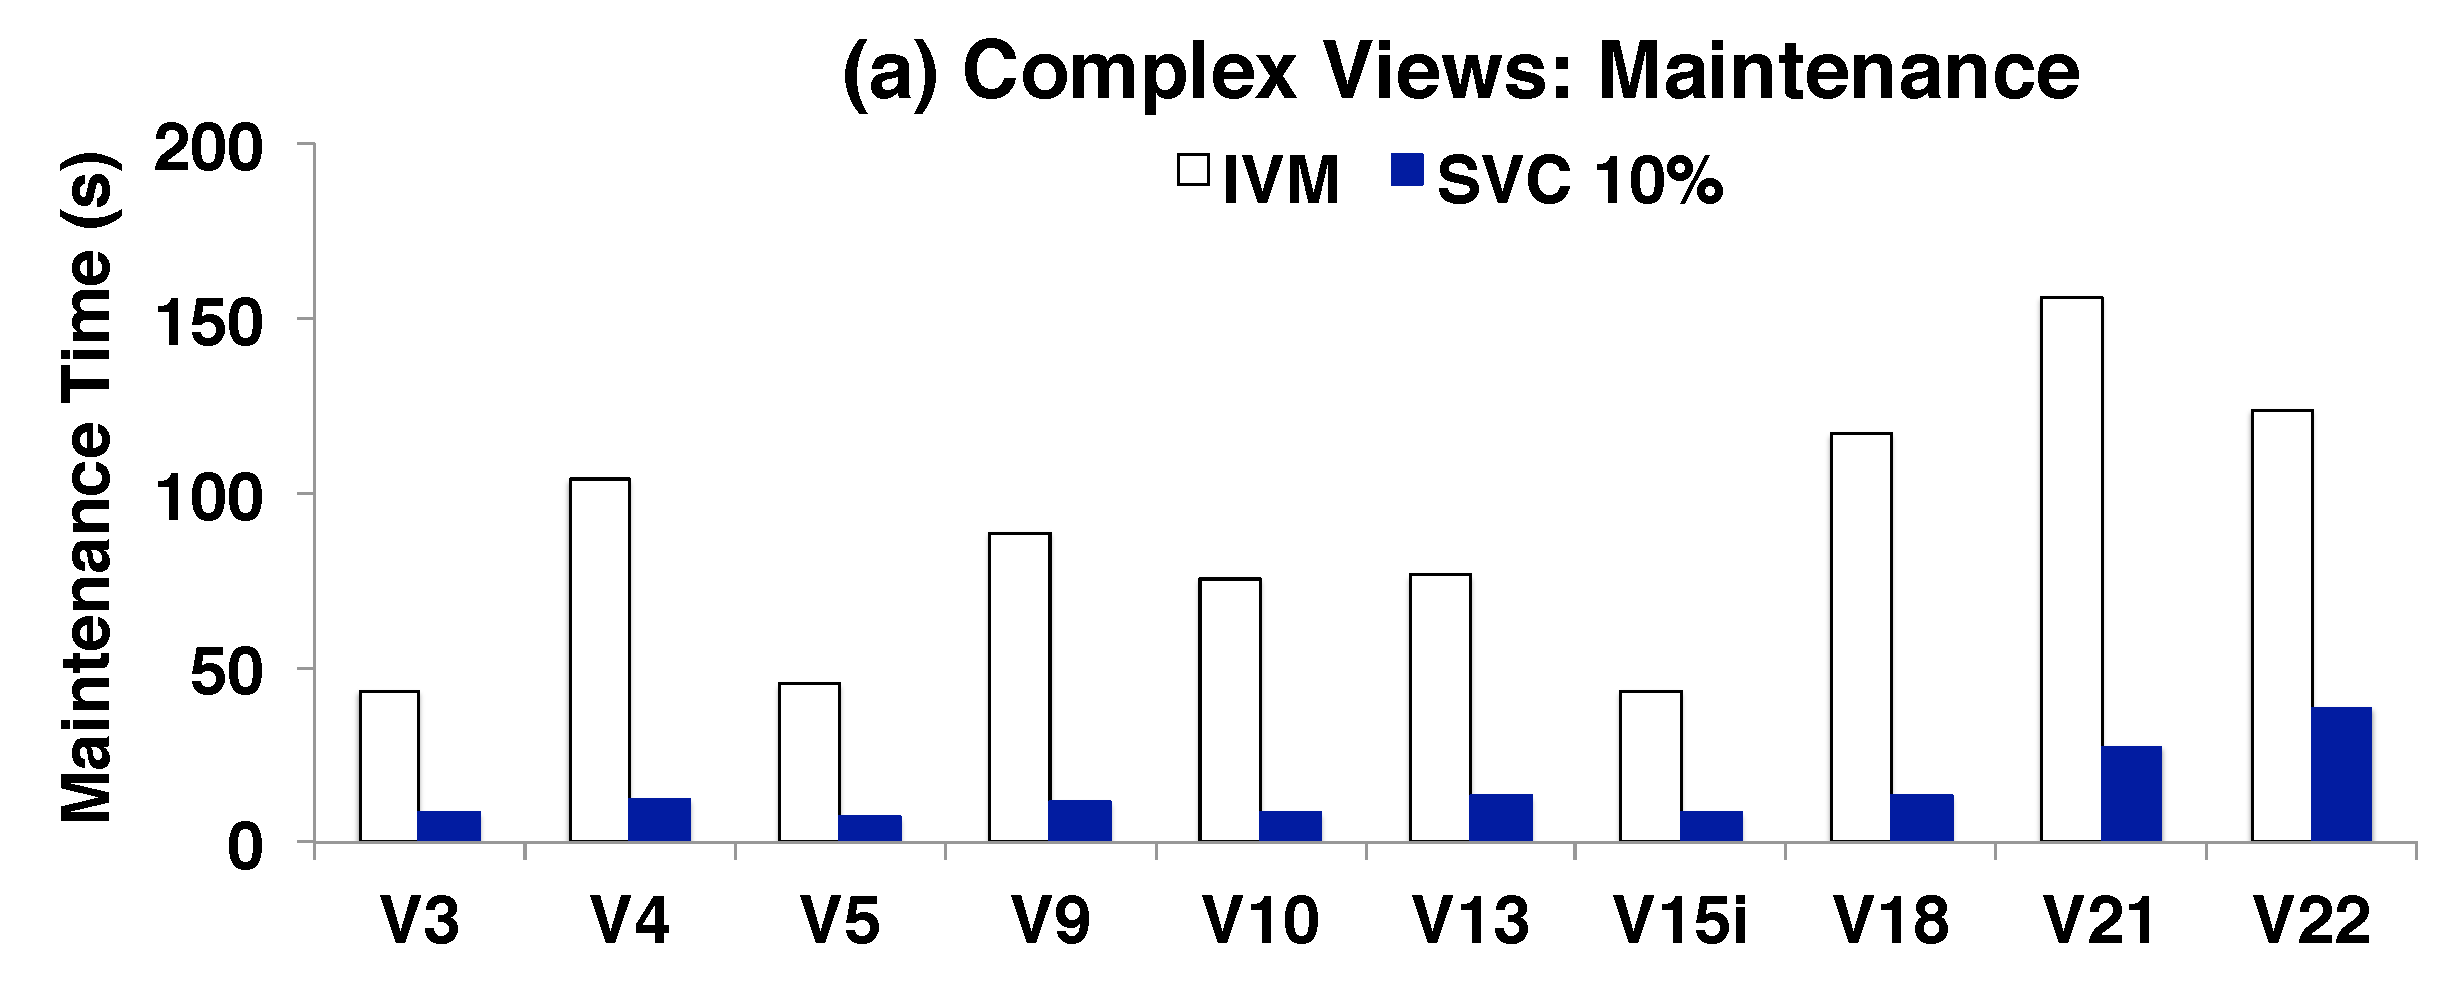
\includegraphics[scale=0.16]{exp/msqv_1.pdf}
 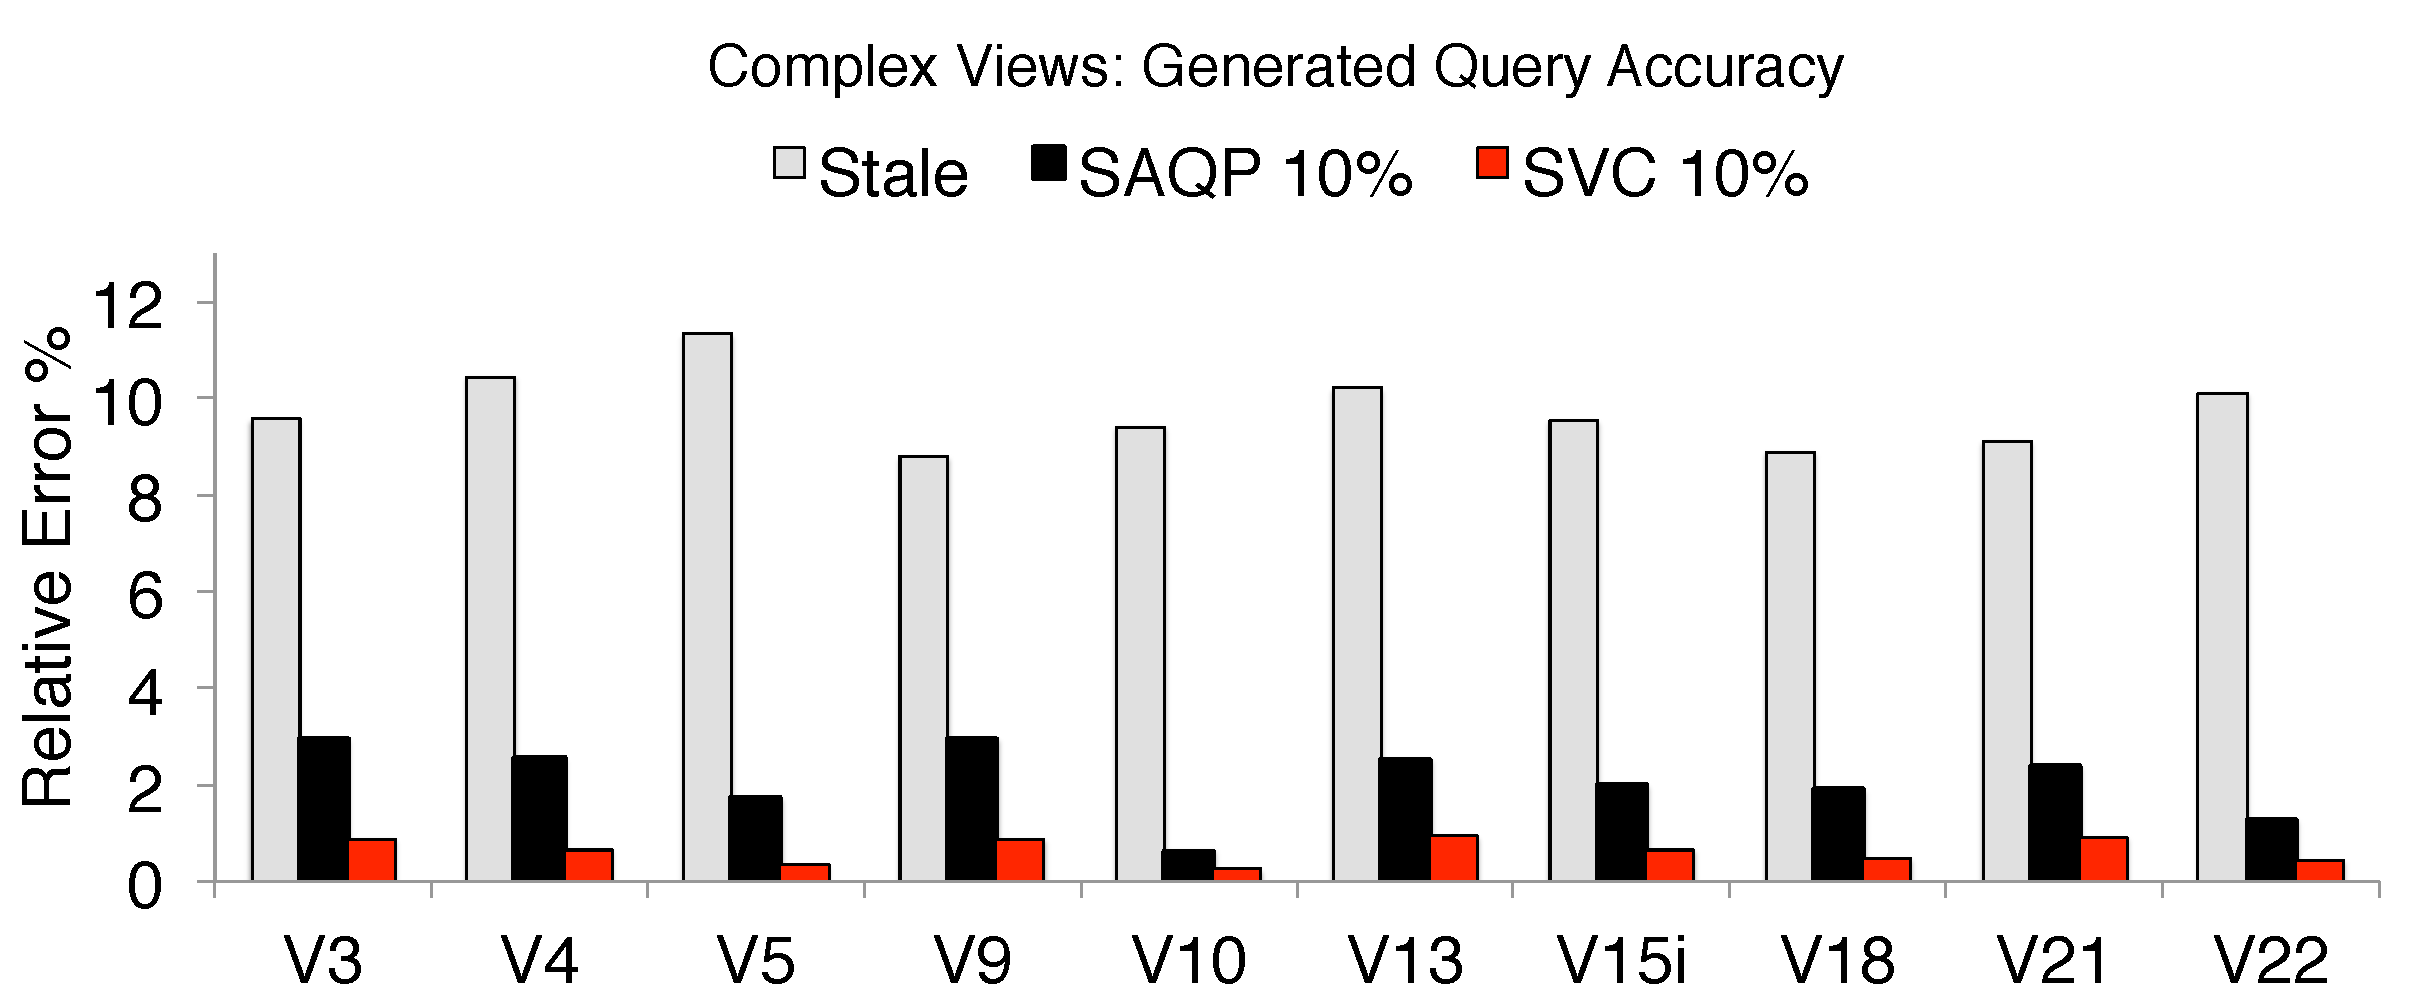
\includegraphics[scale=0.16]{exp/msqv_2.pdf}

 \caption{TODO \label{exp3-acc}}
\end{figure}

The last two experiments picked fixed views and varied the queries on the views.
In this experiment, we demonstrate the breadth of views supported by SVC.
For each of the TPCD queries, we treated these queries as materialized views.
We generated random aggregate queries to run on these views.
We generate a 10GB base TPCD dataset with skew $z=1$ and generate 10 views for
each of the parameterized queries.
Figure \ref{exp3-acc}, shows the maintenance time for a 10\% sample compared to the full view.

For the most part, these results are consistent with our previous experiments showing that SVC is faster than IVM and more accurate than SAQP and no maintenance.
However, this experiment illustrates how the view definitions plays a role in the efficiency of our approach.
For the last two queries, V21 and V22, we see that sampling does not lead to as large of speedup indicated in our previous experiments.
This is because both of those views contain nested structures which block the pushdown of our sampling.
There might be a way to derive an equivalent expression that could be sampled more efficiently, and we will explore this in future work.

\subsubsection{Outlier Indexing}

\begin{figure}[t]
\centering
 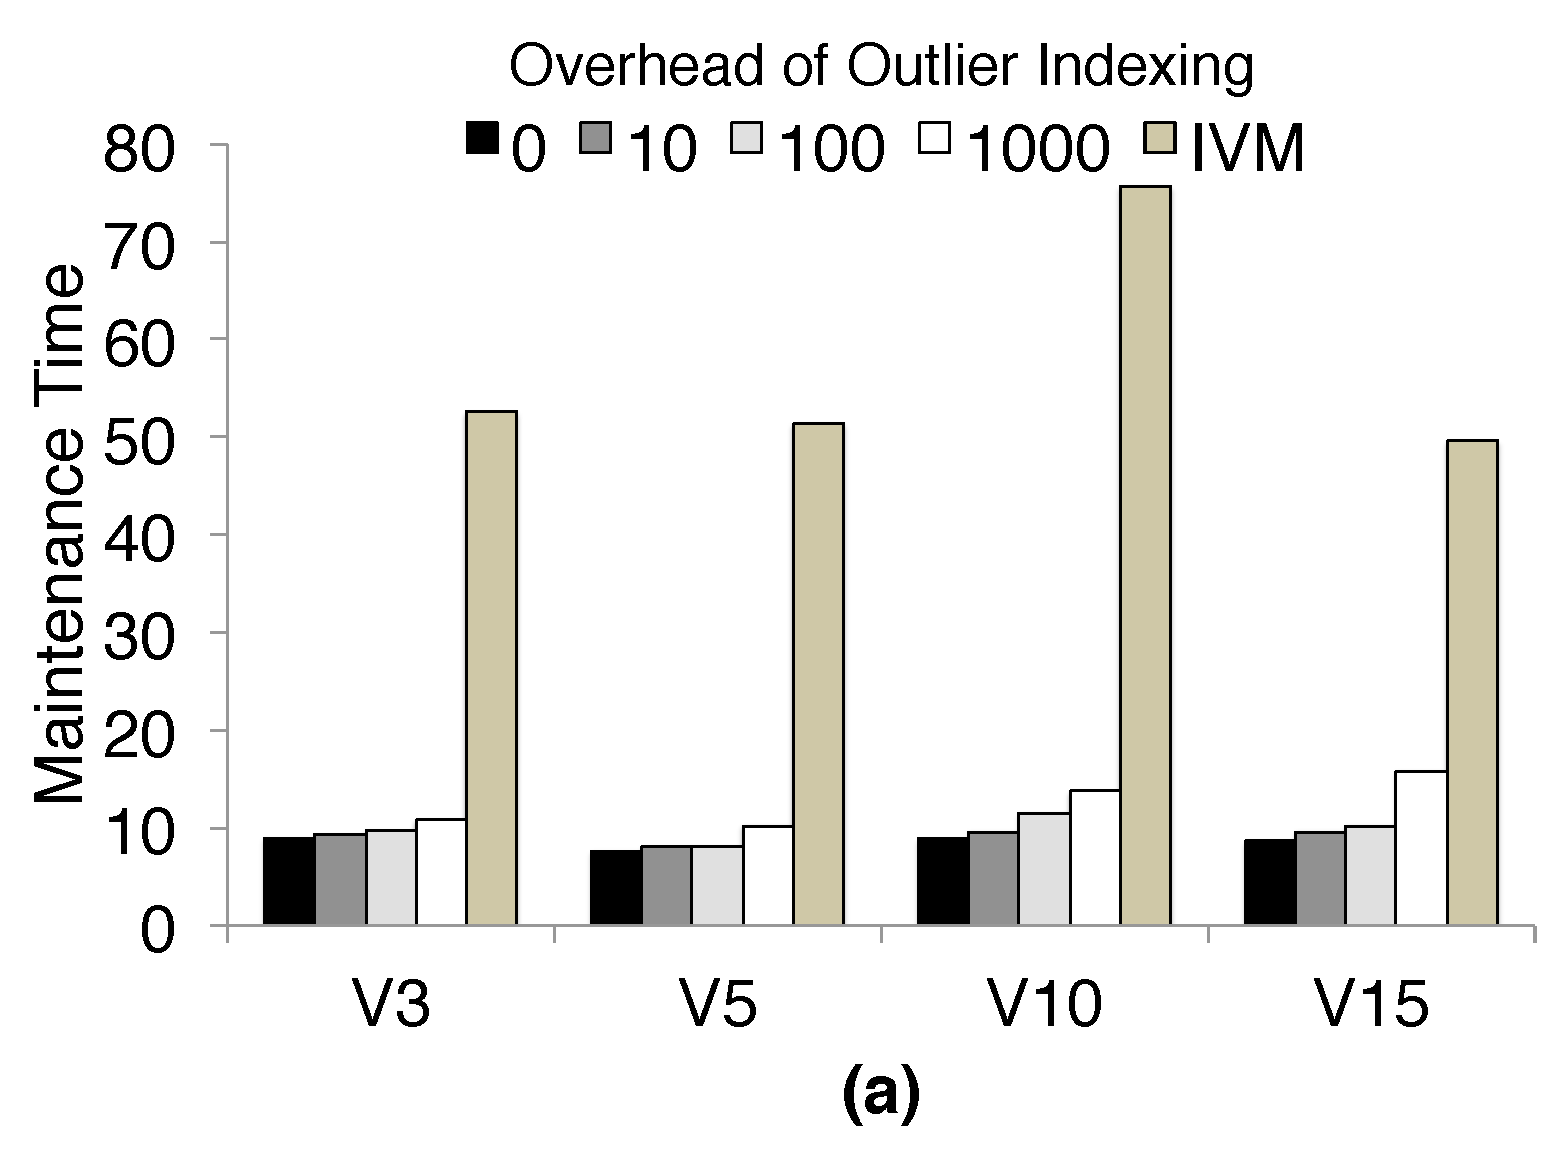
\includegraphics[scale=0.14]{exp/msoi_1.pdf}
 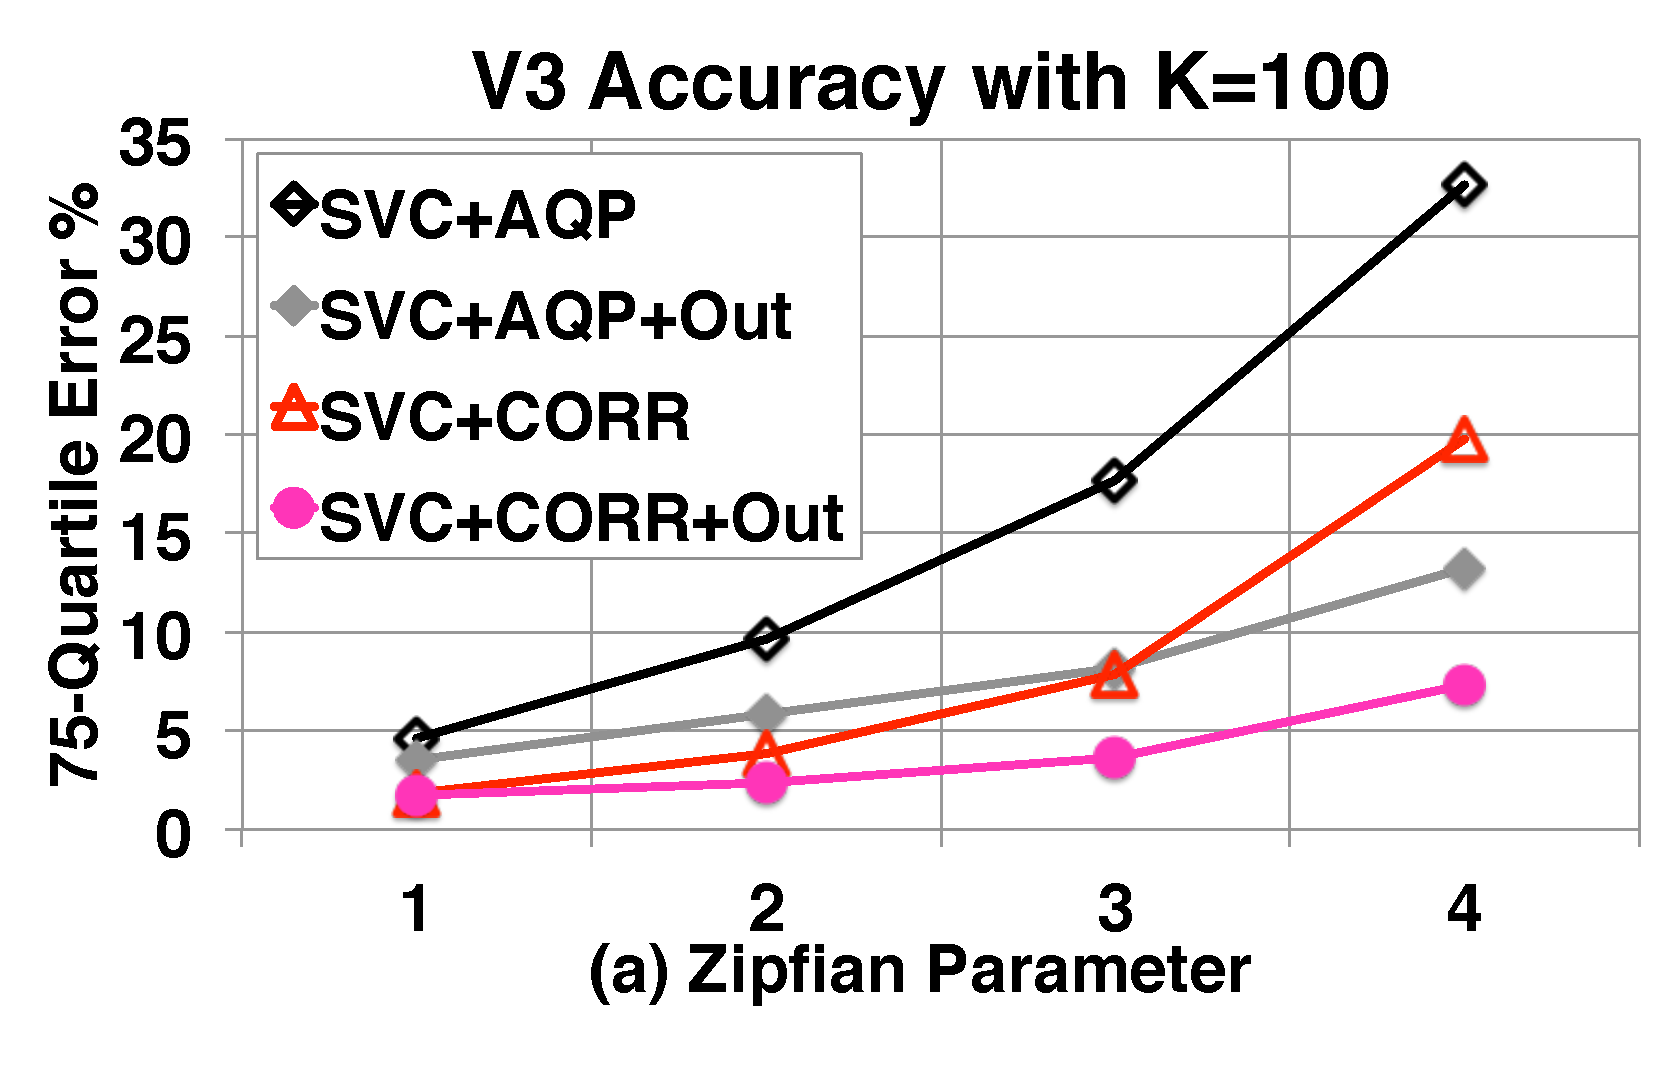
\includegraphics[scale=0.14]{exp/msoi_2.pdf}

 \caption{TODO \label{exp5-oi}}
\end{figure}
We hinted at the sensitivity to dataset skew of sampling-based approaches ealier.
In our next experiment, we evaluate our outlier indexing.
Our outlier indices are constructed on the base relations.
We index the \textbf{l\_extendedprice} attribute in the \textbf{lineitem} table.
We evaluate the outlier index on the TPCD query views.

We find that four views: V3, V5, V10, V15, can benefit from this index with our push-up rules.
We set an index of 100 records, and applied SVC to datasets with skew parameter $z=\{1,2,3,4\}$. 
We run the same queries as before, but this time we measure the error at the 75\% quartile.
In Figure \ref{exp5-oi} a, we find in the most skewed dataset SVC with outlier indexing reduces query error by a factor of 2.
In the next Figure (Figure \ref{exp5-oi} b), we plot the overhead for outlier indexing for an index size of 0, 10, 100, and 1000.
While there is an overhead, it is still small compared to the gains made by sampling the maintenance strategy.

\subsubsection{Systems Considerations}
\begin{figure}[t]
\centering
 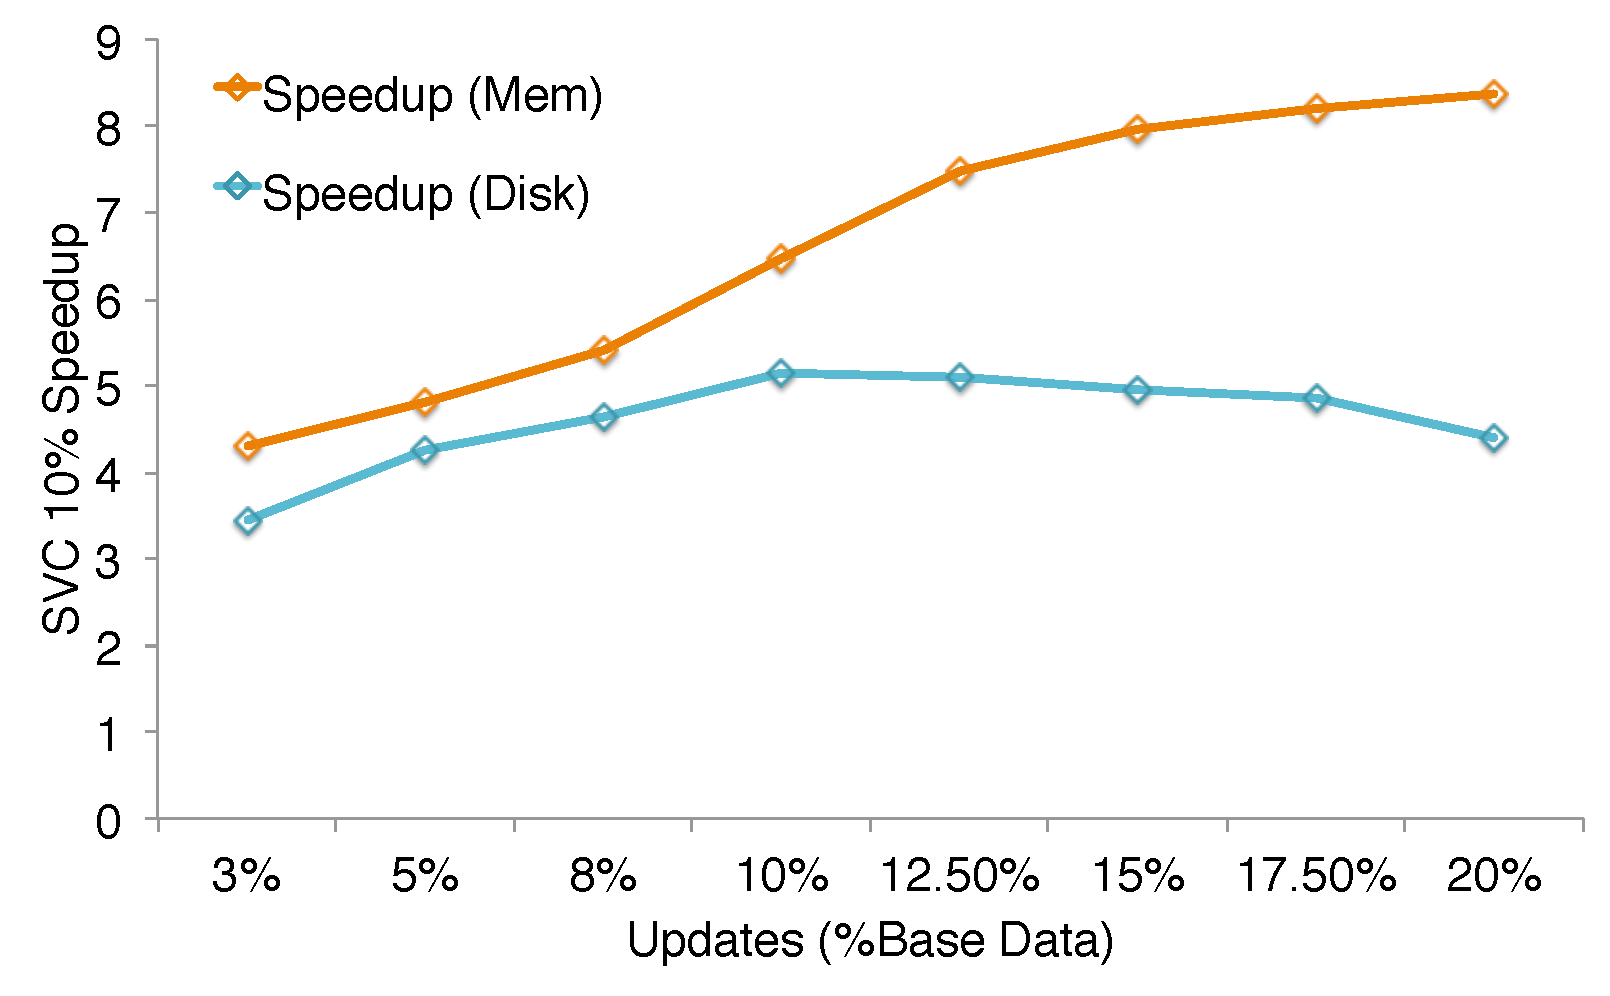
\includegraphics[scale=0.14]{exp/mssd_2.pdf}
 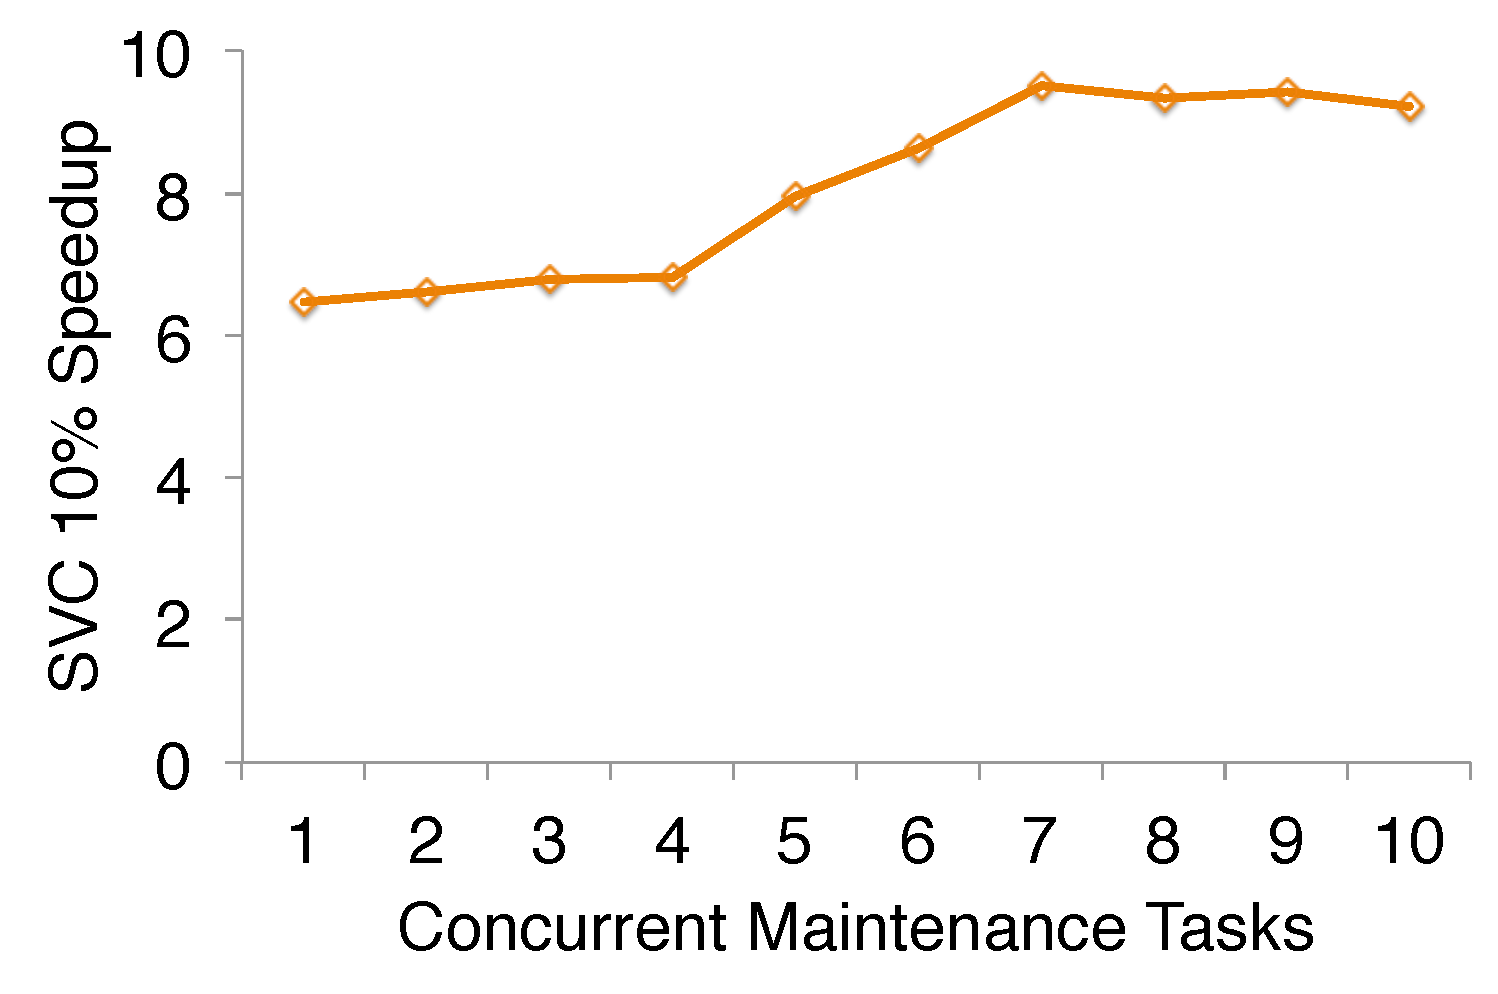
\includegraphics[scale=0.14]{exp/mssd_1.pdf}

 \caption{TODO \label{exp6-sys}}
\end{figure}

We also explored how different system characteristics affect the efficiency of SVC.
In Figure \ref{exp6-sys}, we took the data cube base view and applied SVC to it.
We compared placing the updates to the view in memory and on disk, and varied the size of the updates.
For the in-memory version, as the updates increased, SVC becomes more efficient.
On the other hand, when the data is on disk the benefits level off and actually decrease as both SVC and IVM have to 
expend the same I/O cost of loading the data into memory.
In a real system with multiple views, this cost can be amortized over all views.
In Figure \ref{exp6-sys}, we also ran maintenance tasks in parallel threads.
We found that as contention for the CPU increased the benefits of SVC also increased.
SVC is most beneficial when maintenance is CPU-bound.

\subsection{Conviva}
In our next set of experiments, we applied SVC to a 1TB dataset of logs from Conviva Inc.
This dataset was given to us in denormalized form.
We also recieved a workload of queries corresponding to this dataset.
In this workload, there were annotated summary statistics queries, and we filtered for the most common types.
While, we cannot give the details of the queries, we can present some of the high-level characteristics.
\begin{itemize}
\item \textbf{1. ErrAnal:Summary} Counts of various error types grouped by resources, users, date
\item \textbf{2. DmsRpt:UsageSum} Sum of bytes transfered grouped by resource, users, date
\item \textbf{3. DmsRpt:SaveSum} Counts of visits grouped by an expression of resource tags, users, date.
\item \textbf{4. CdnRpt:cdnSum} Nested query that groups users from similar regions/service providers together then aggregates statistics
\item \textbf{5. ErrorDetails} Nested query that groups users from similar regions/service providers together then aggregates error types
\item \textbf{6. EngageRpt:HD} Union query that is filtered on a subset of resources and aggregates visits and bytes transfered
\item \textbf{7. IntegRpt:Summary} Group by resources, users, date with many aggregates.
\item \textbf{8. EngageRpt:Q1} Group by resources, users, date with many aggregates.
\end{itemize}
We treat these queries as materialized views to evaluate SVC.
We implement SVC on a 10-node Spark cluster.

\subsubsection{Performance and Accuracy}
\begin{figure}[t]
\centering
 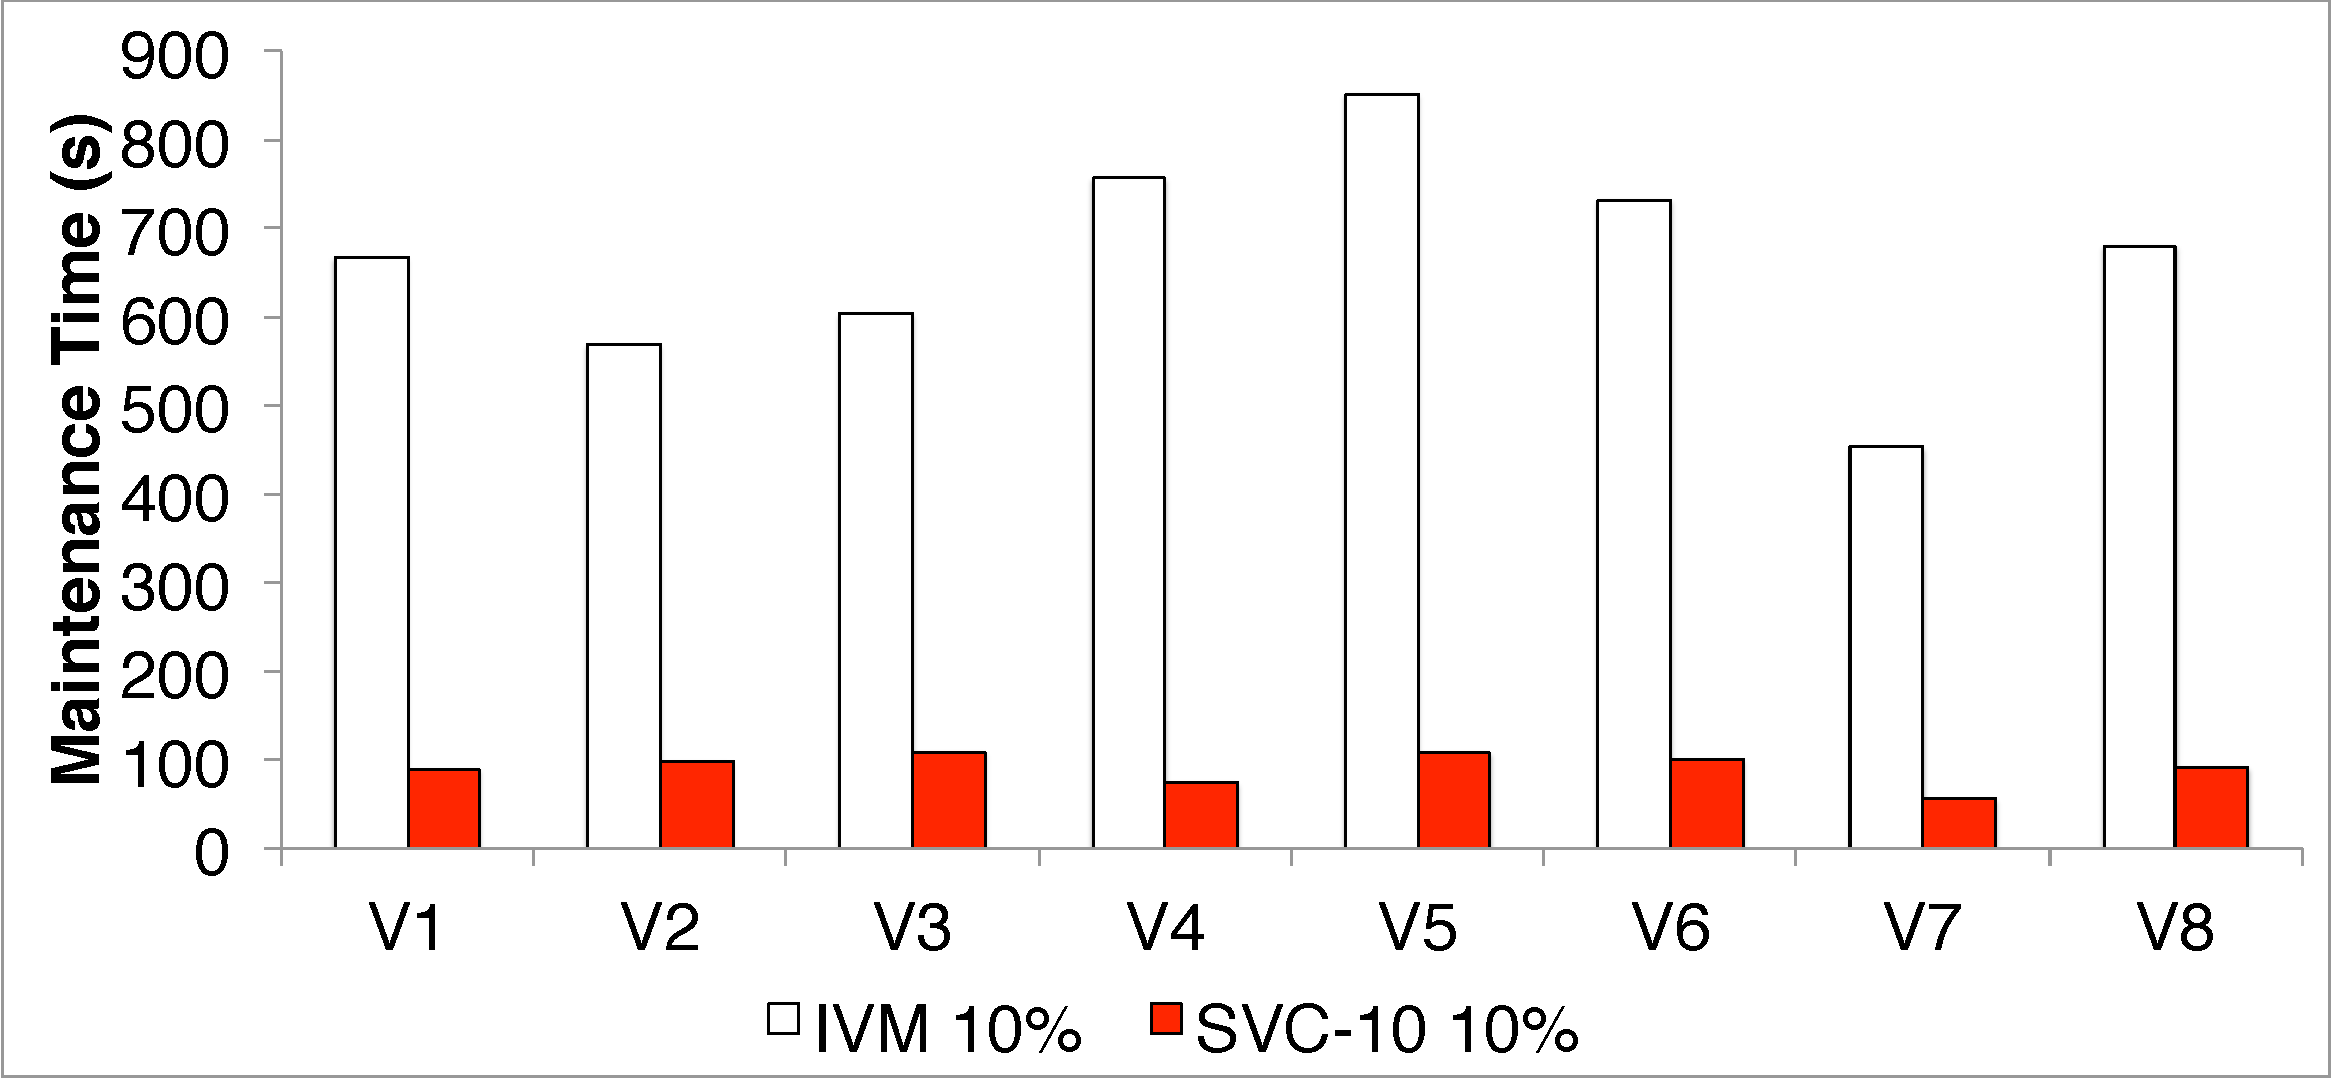
\includegraphics[scale=0.14]{exp/con_2.pdf}
 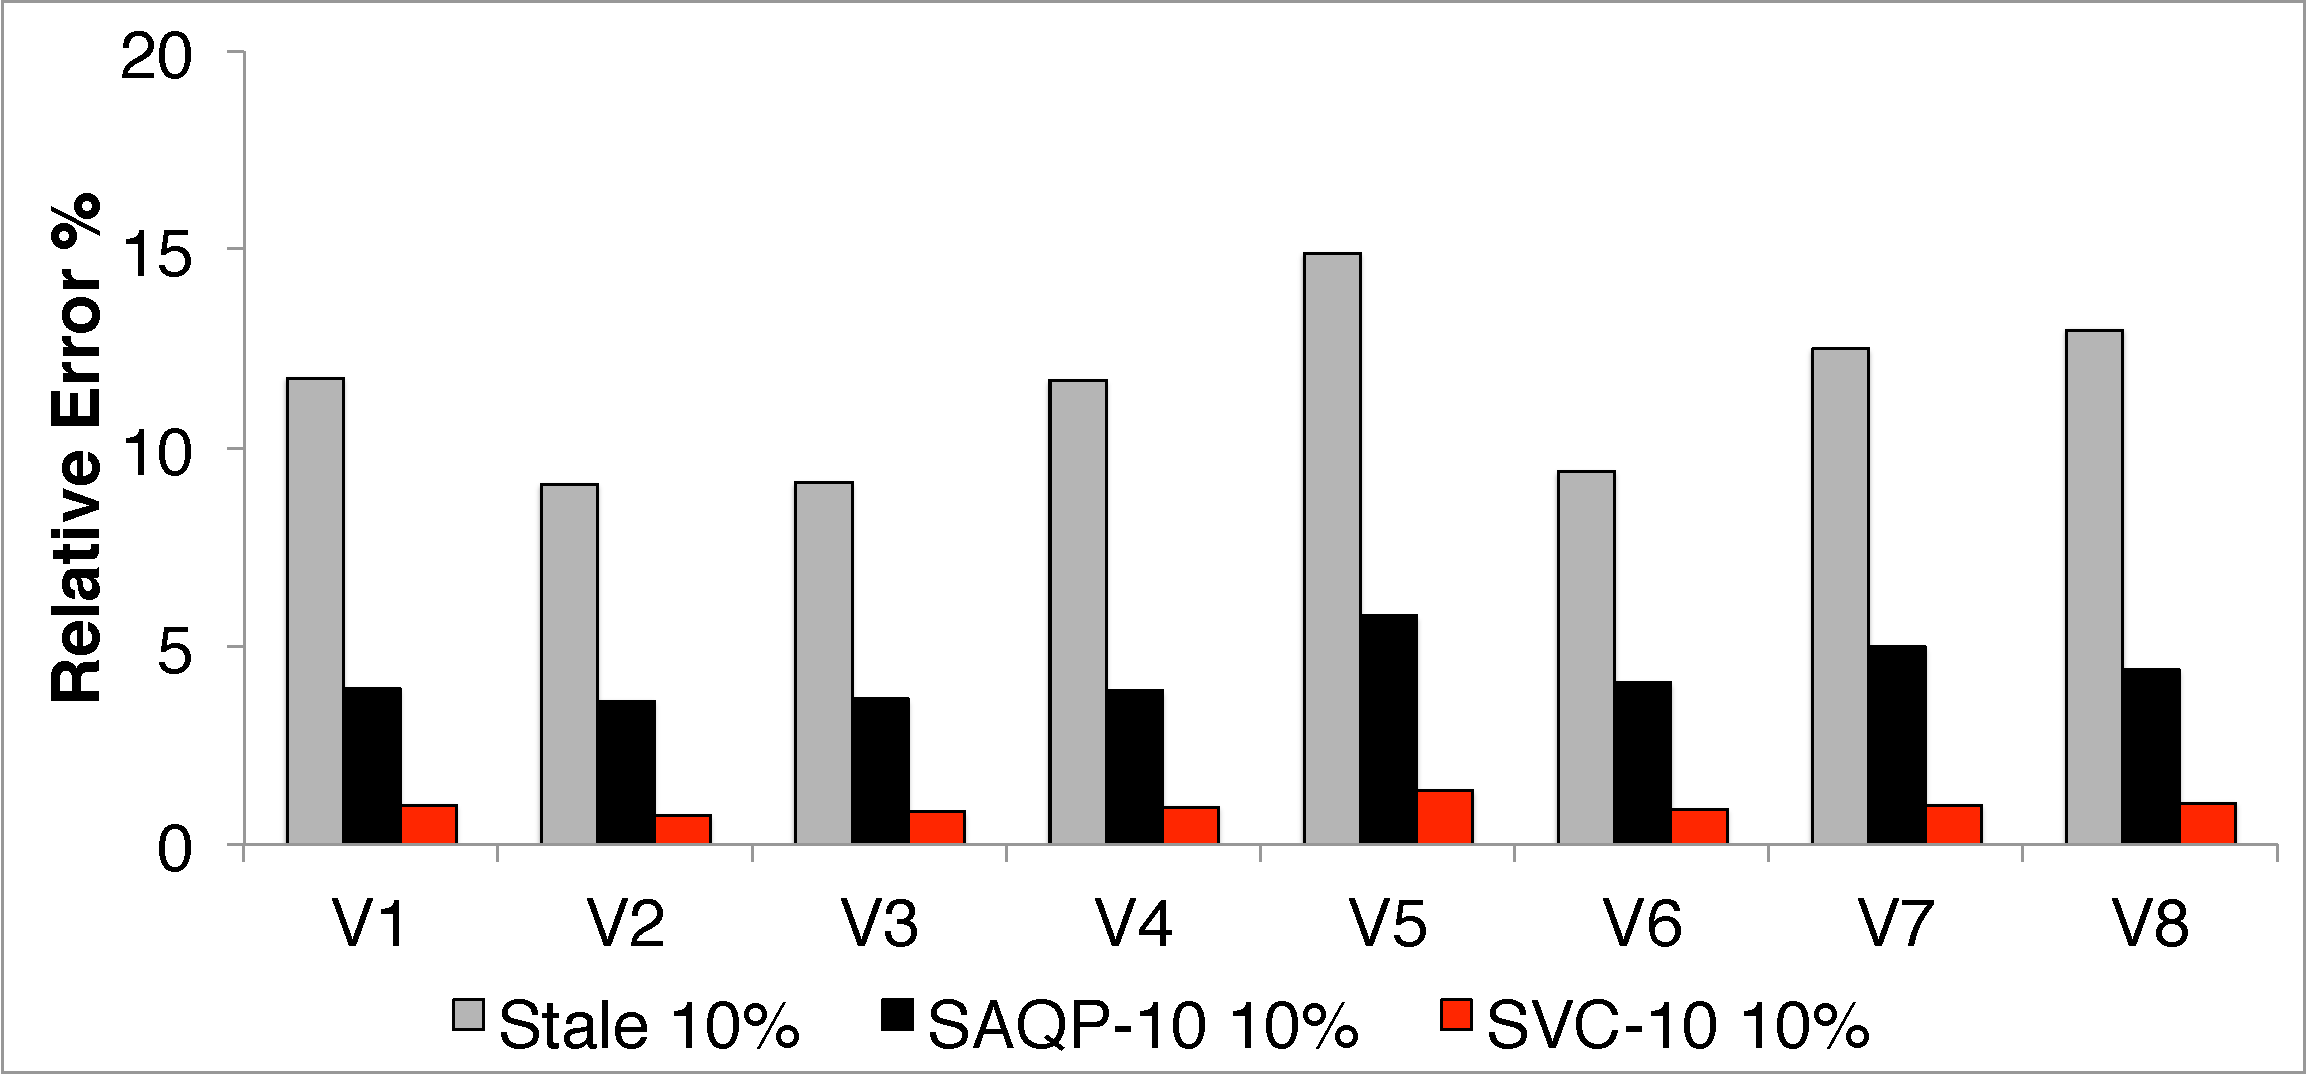
\includegraphics[scale=0.14]{exp/con_1.pdf}
 \caption{TODO \label{conv-1}}
\end{figure}
We derive these views from 800GB of base data and add 80GB of updates.
In Figure \ref{conv-1}, we show that while full maintenance takes nearly 800 seconds for one of the views, a 10\% SVC can complete sample maintenance in less than 100s for all of them.
SVC also gives highly accurate results with an error of 0.98\%.
In the following experiments, we will use V2 and V5 as exemplary views.
V5 is the most expensive to maintain due to its nested query and V2 is a single level group by aggregate.
These results show consistency with our results on the synthetic datasets.

\subsubsection{End-to-end integration with periodic maintenance}
\begin{figure}[t]
\centering
 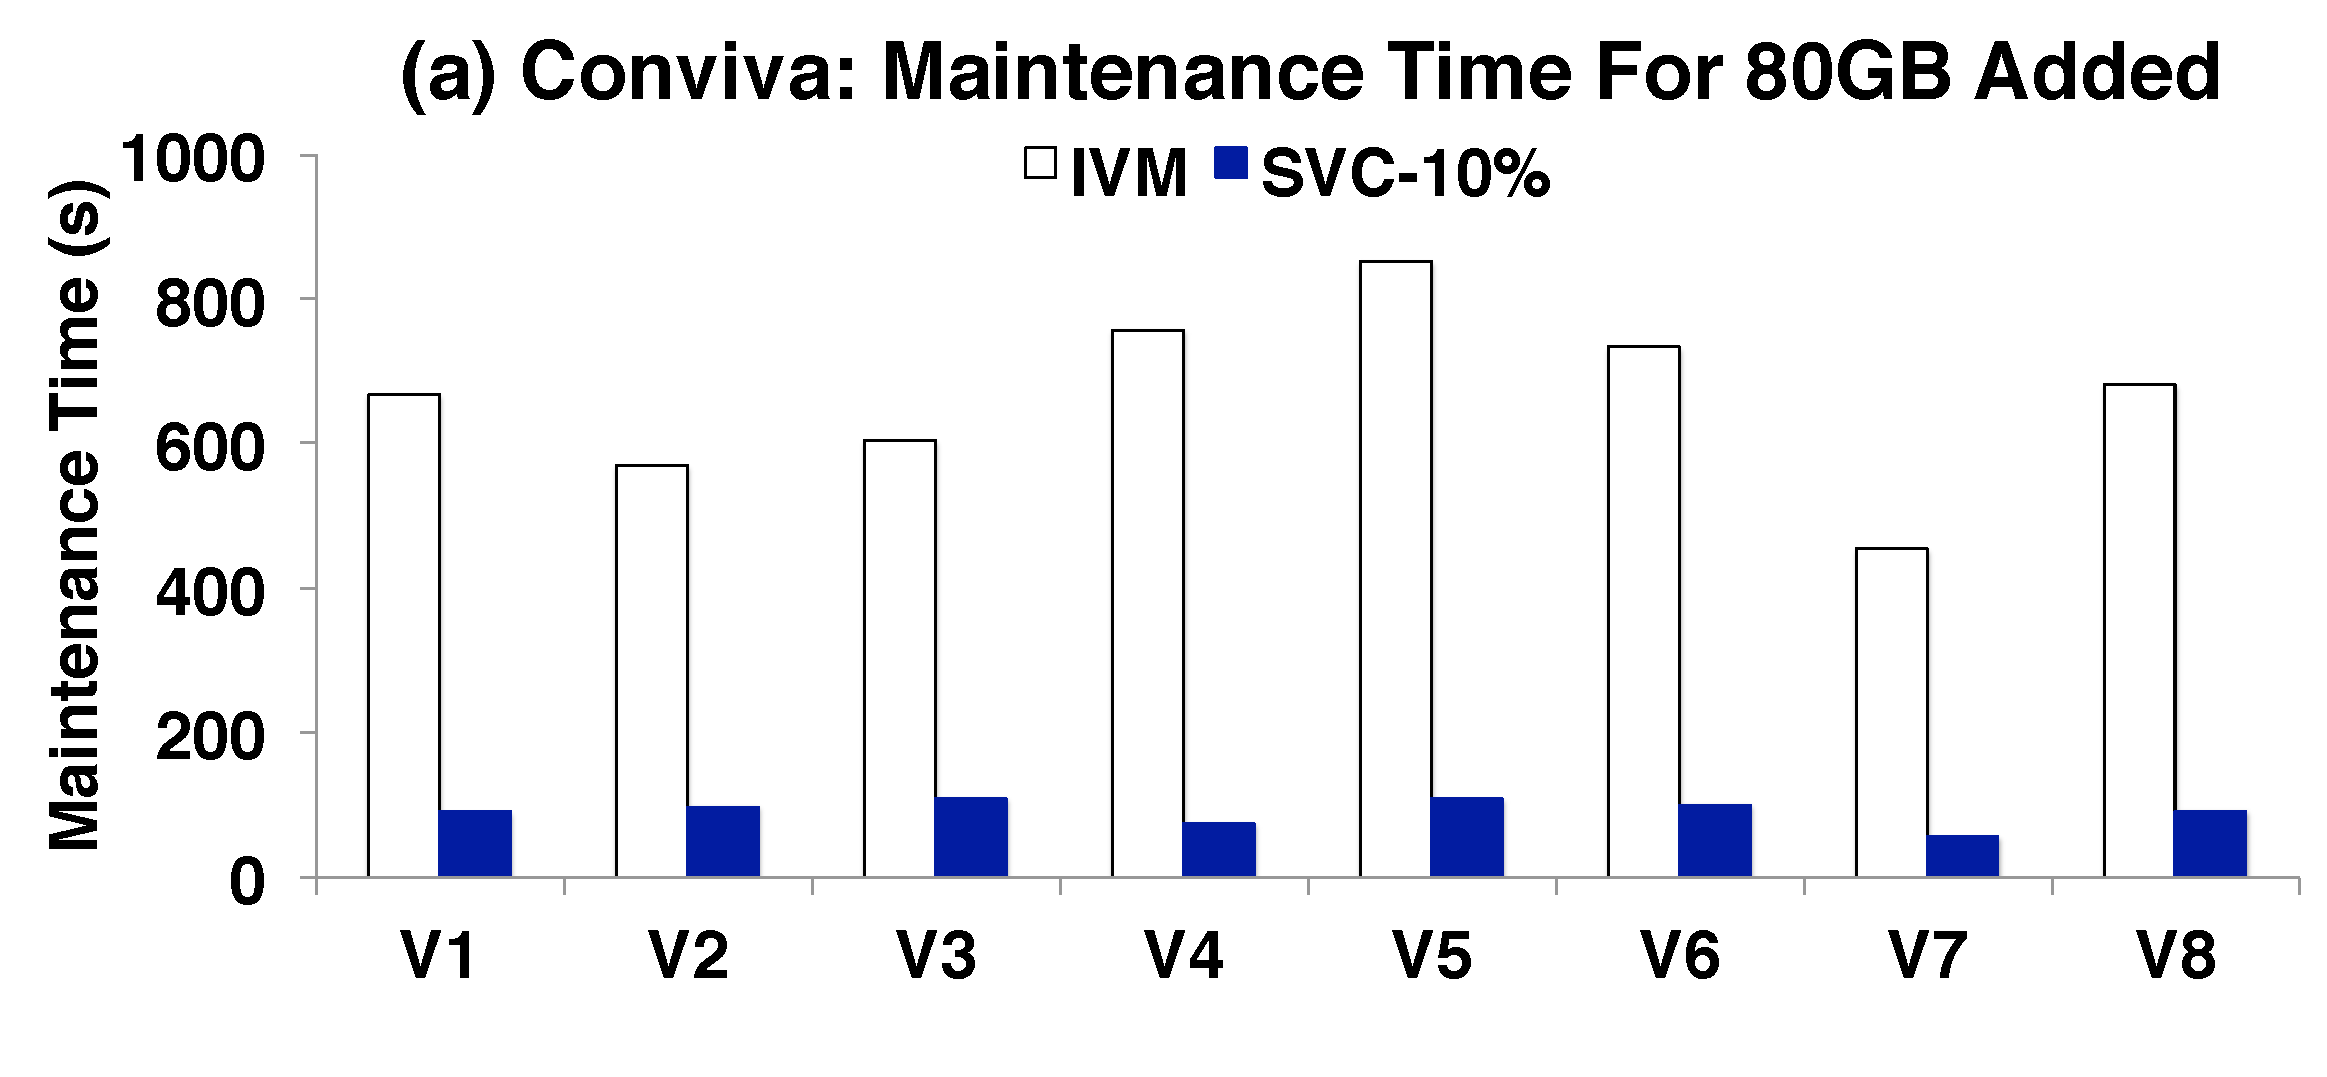
\includegraphics[scale=0.14]{exp/con_3.pdf}
 \caption{TODO \label{conv-2}}
\end{figure}

\begin{figure}[t]
\centering
 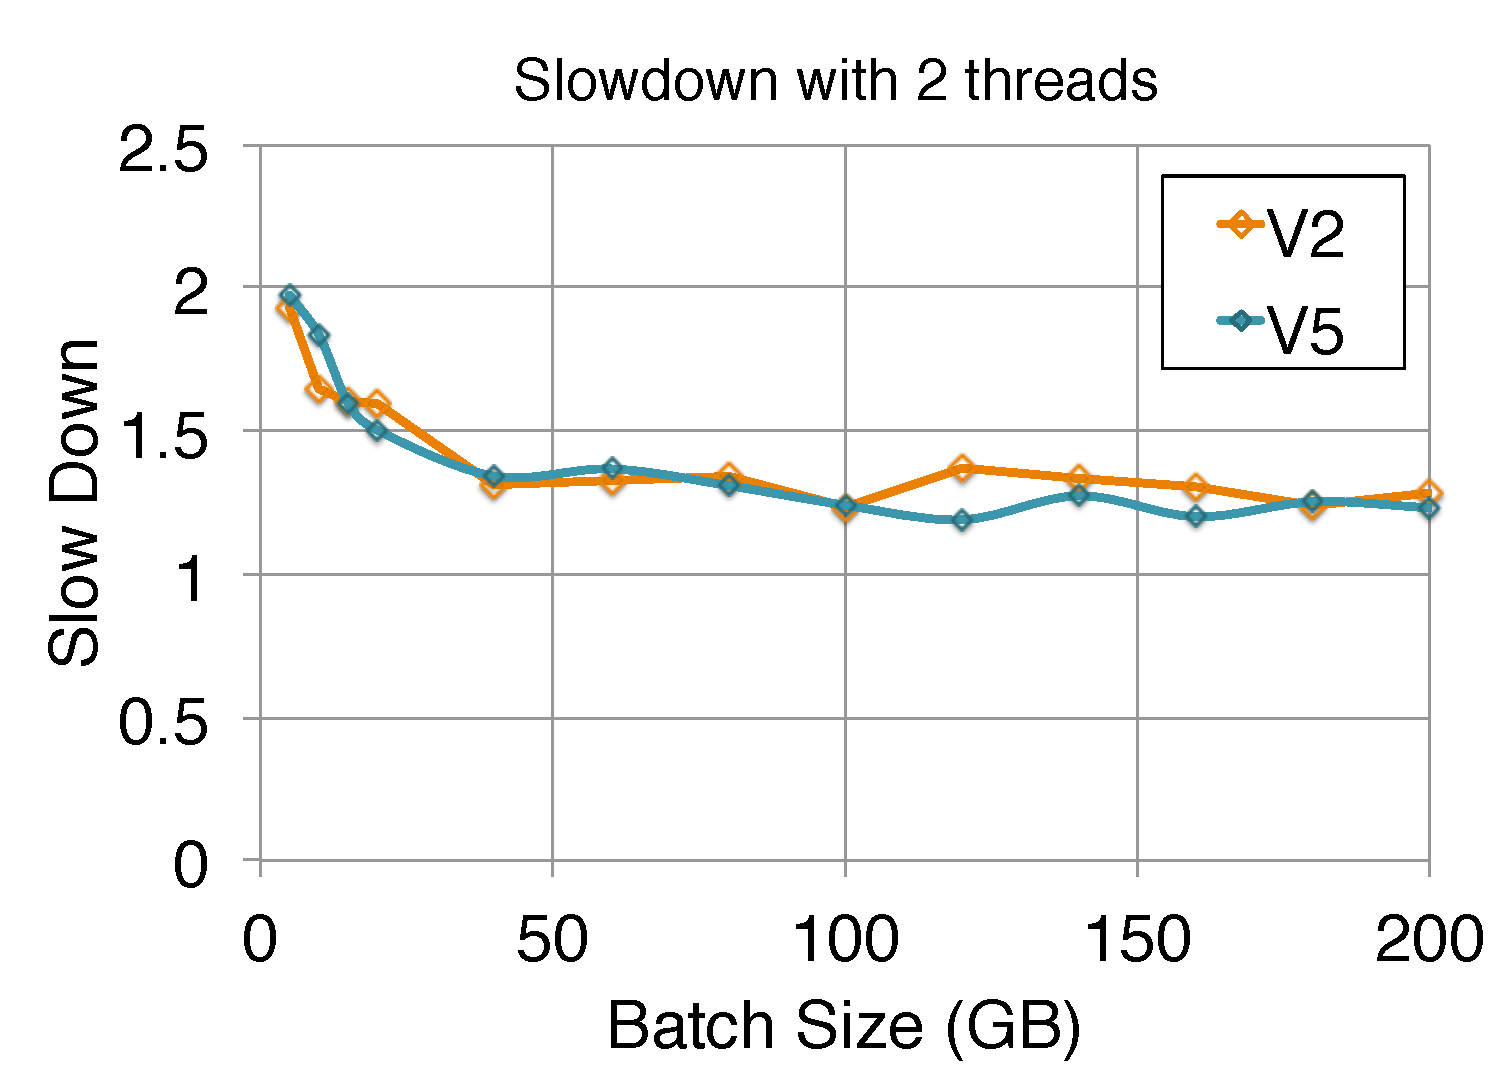
\includegraphics[scale=0.14]{exp/con_4.pdf}
 \caption{TODO \label{conv-3}}
\end{figure}

We devised an end-to-end experiment simulating a real integration with periodic maintenance.
However, unlike the MySQL case, Apache Spark does not support selective updates and insertions as the ``views" are immutable.
A further point is that the immutability of these views and Spark's fault-tolerance requires that the ``views" are maintained synchronously.
Thus to avoid these significant overheads, we have to update these views in batches.
In Figure \ref{conv-2}, we show a tradeoff between batch size and throughput of Spark for V2 and V5.
Throughputs for small batches are nearly 10x smaller than the throughputs for the larger batches.

We can apply SVC in a batch mode as well.
In implementation, we can exploit on key aspect of SVC.
Since it only maintains a sample, we need not touch the immutable view and keep the immutable data structures
distinct.
Therefore, we can run SVC and a periodic maintenance task in concurrent threads.

In this model, there are a lot of different parameters: batch size for periodic maintenance, batch size for SVC, sampling ratio for SVC, and the fact that concurrent threads may reduce overall throughput.
We chose these parameters in the following way.
First, we measure the reduction in throughput when running multiple threads.
This is shown in Figure \ref{conv-3}, where we plot the reduction in throughput against batch sizes.
Larger batch sizes are more amenable to parallel computation.

\begin{figure}[t]
\centering
 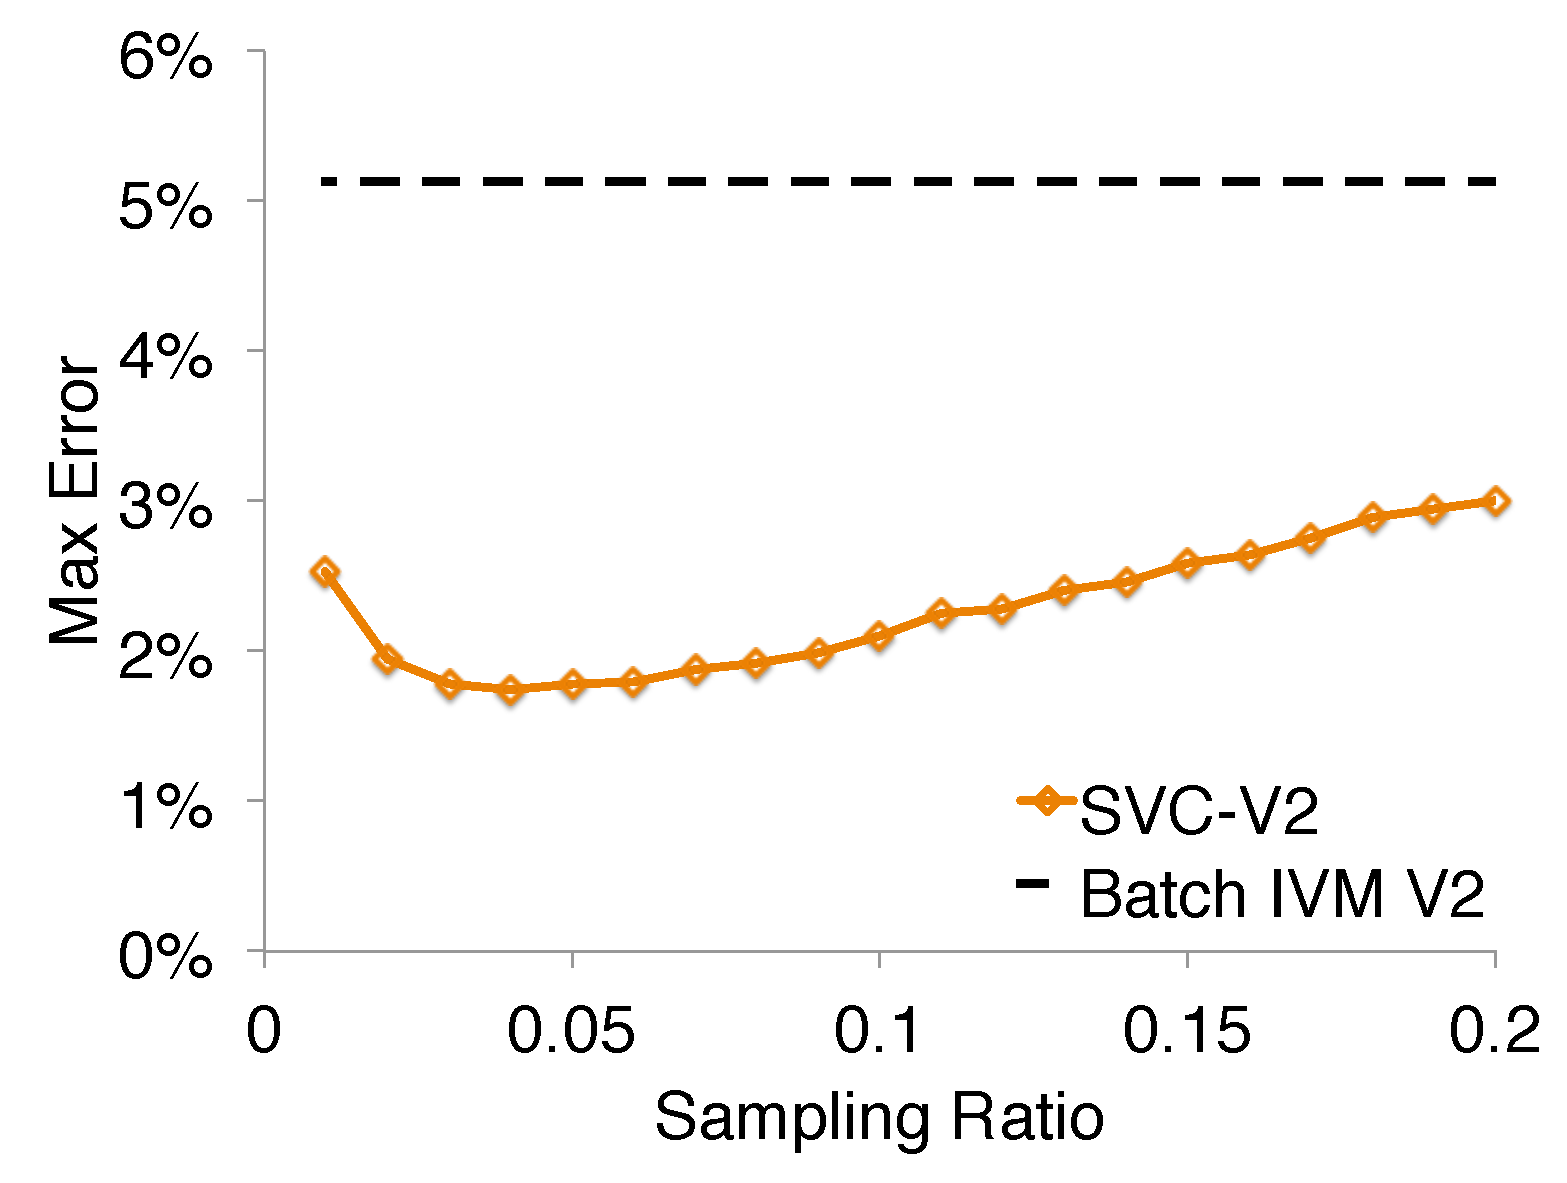
\includegraphics[scale=0.14]{exp/con_5.pdf}
 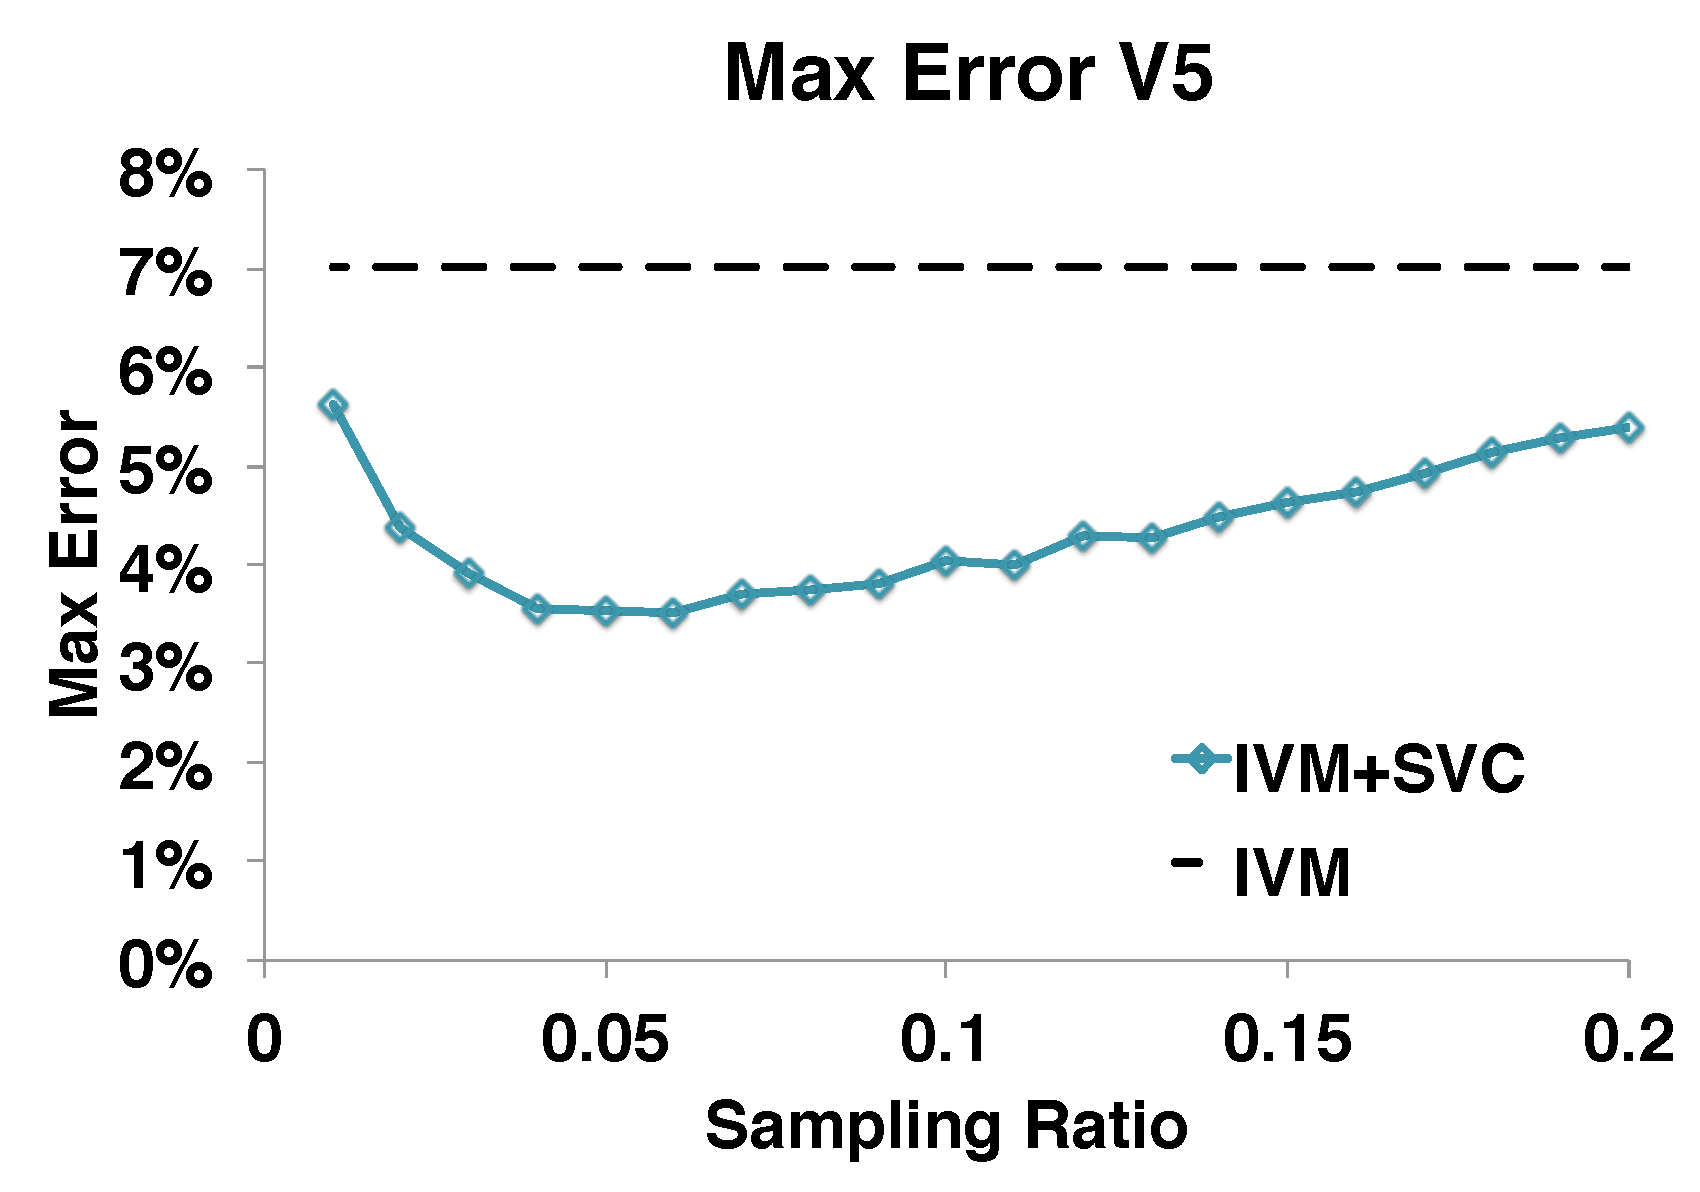
\includegraphics[scale=0.14]{exp/con_6.pdf}
 \caption{TODO \label{conv-4}} 
\end{figure}

Using this, we set a throughput demand for both periodic maintenance and svc+periodic maintenance.
For V2, this was set at 700,000 records/sec and for V5 this was 500,000 records/sec.
For this fixed throughput, we chose the smallest batch size for each approach that satisfies the throughput.
When running periodic maintenance alone view updates can be more frequent, and when run in conjunction with SVC it is less frequent.

Within the SVC period, we run our sample maintenance on a loop continously updating the sample view.
There is further a tradeoff with the sample size, larger samples give more accurate estimates however between SVC batches they go stale.
We quantify the error in these approaches with the max error; that is the maximum error in a maintenance period (Figure \ref{conv-4}).
These competing objective lead to an optimal sample size of 3\% for V2 and 6\% for V5.
At this sampling point, we find that applying SVC gives results 2.8x more accurate for V2 and 2x more accurate for V5.

\begin{figure}[t]
\centering
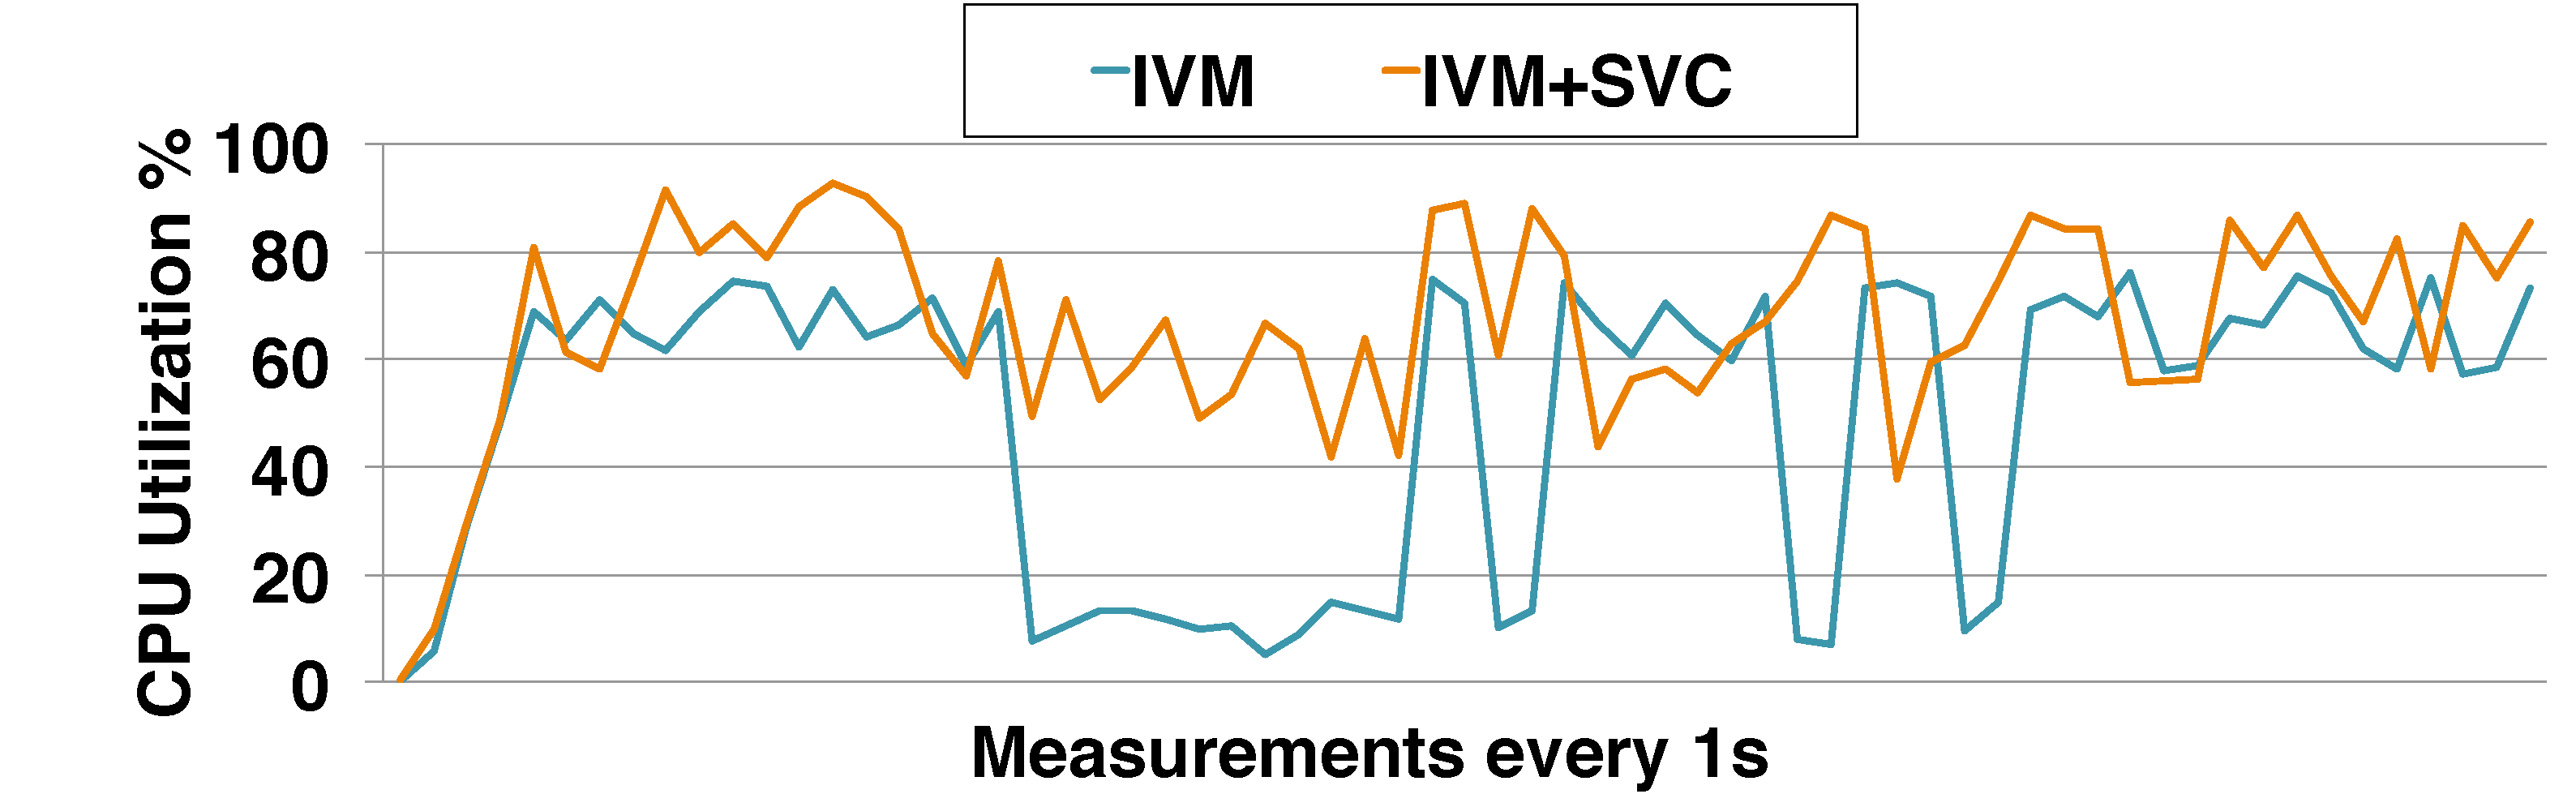
\includegraphics[scale=0.14]{exp/con_7.pdf}
 \caption{TODO \label{conv-5}} 
\end{figure}
To give some intuition on why SVC gives more accurate results, in Figure \ref{conv-5}, we plot the average CPU utilization of the cluster for both periodic maintenance and svc+periodic maintenance. 
We find that SVC takes advantage of the idle times in the system; which are common during shuffle operations in a synchronous parallelism model.

In a way, these experiments present a worst-case application for SVC, yet it still gives improvements in terms of query accuracy.
In many typical deployments throughput demands are variable forcing maintenance periods to be longer eg. nightly.
The same way that SVC takes advantage of micro idle times during communication steps, it can provide large gains during controlled idle times when no maintenance is going on concurrently.


